\section{Моделът \texorpdfstring{$\aDg$}{αDg}} 
Преди всичко, да въведем обозначенията, които ще използваме. Нека $\sigma_0$ бъде началното пресищане (за $t = 0 $) на разтвора (преди кристали да са се образували). Нека тогава $\sigma = \sigma(t)$ бъде пресищането в даден момент от време $t > 0$. Тогава дефинираме относителното пресищане като:
\begin{equation*}
	\Theta \coloneqq \frac{\sigma}{\sigma_0}
\end{equation*}
Така $\Theta \in [0,1]$ и е безразмерна величина, характеристична за моментното състояние на процеса.

Ще въведем и $r$  - магнитуда на нормалната скорост, с която кристалната стена напредва в разтвора. Съответно, $r_0$ ще е стойността на $r(t=0)$, която ще бъде важна скала при обезразмеряване на уравненията, които ще бъдат изведени по-долу.

Степента на превръщане $\alpha$, която беше / в контекста на JMAKn, сега ще дефинираме като:
\begin{equation}
	\label{eq:alpha_ndef_def}
	\alpha \coloneqq \frac{N(t)}{N_{max}}
\end{equation}
Където $N(t)$ е броят растящи кристали в момента $t$ и $N_{max}$ е максималният брой кристали, които ще се образуват при достигане на равновесие.

Ако предположим, че имаме $\eta$ кристала растящи едновременно, които не си взаимодействат през дифузионните си полета, тогава можем да дефинираме $\alpha$ през $D$-мерният обем на кристала. В такъв случай общото пресищане ще бъде разделено на броя растящи кристали поравно.

\begin{equation}
	\label{eq:alpha_vol_def}
	\alpha \coloneqq \frac{V(t)}{V_{max}}
\end{equation}
$\alpha \in [0,1]$ и също е безразмерна величина.

\subsection{Получаване на основното ОДУ на модела}
Стратегията за извеждане на основното ОДУ на модела ще бъде като започнем от следната форма на закона за запазване на масата:
\begin{equation}
	\label{eq:mass_conservation_law}
	\alpha(t) = 1 - \Theta(t)
\end{equation}
\noindent Физическият смисъл на \autoref{eq:mass_conservation_law} е следният: една частица може да е или в разтвора и да допринася за относителното пресищане или да е в кристала и да допринася за степента на превръщане.

Нататък продължаваме с основното следствие от BCF-модела \cite{BCF1951} и го комбинираме с \autoref{eq:mass_conservation_law}:
\begin{equation}
	\label{eq:bcf_corollary}
	r = r_0(g)(1-\alpha)^g
\end{equation}
Където $g$ е параметър от BCF модела. Каноничните стойности за $g$ са \textit{1} в режима на бърза кинетика (дифузионно контролиран растеж) и \textit{2} за кинетично контролиран.

\autoref{eq:bcf_corollary} записано в този вид напомня на закона за действие на масите (ЗДМ) на  \textit{Гулдберг и Вааге} и по тази причина параметърът $g$ понякога се нарича \textit{порядък на растеж}. Тук следва да се отбележи, че трябва тази аналогия със ЗДМ да се ползва внимателно, тъй като в лявата страна на уравнението $r$ е скоростта на фронта, а не производна на концентрацията (скорост на химична реакция - chemical rate). Още повече, това движение на кристалната стена е ефективно - всяка свързала се единица остава фиксирана към нея.

\noindent Общата скорост на растеж се дефинира като:
\begin{equation}
	\label{eq:overall_growth_rate}
	G \coloneqq \frac{dl}{dt}
\end{equation}
Където $l$ - линеен характеристичен размер на кристала (напр. полудължина на нишката при едномерен растеж, страна на квадрат при двумерен, страна на куб при тримерен).
При т.нар. \textit{полиедричен} растеж всеки две срещуположни стени нарастват едновременно спрямо центъра (началния зародиш). Т.е. общата скорост на растеж е два пъти скоростта на напредване на стената: $G = 2r$, за да се запази полиедричната форма на кристала.
В експерименти, при които пресищането се довежда до своята максимална стойност в началото и след това не се поддържа допълнително, както и допълнителното зародишообразуване е потиснато (напр. двойно-импулсната техника) фиксиран малък брой кристали $\eta$ растат и имат един и същ характеристичен размер $l$. Това ни позволява да разглеждаме случая, когато кристалите не си взаимодействат с дифузионните си полета. Допълнително, в такива условия е по-вероятно дифузията да е бавна и съответно $g = 1$.

Растежът приключва когато кристалите достигнат своята максимална характеристична дължина $l_{max}$. Може да се покаже чрез анализ на размерностите за $l_{max}$ \cite{Tsoularis2002}:
\begin{equation}
	\label{eq:l_max}
	l_{max} = f\left(N^{-\frac{1}{D}}, (c-c_{eq}) \right)
\end{equation}
Ще обезразмерим \autoref{eq:overall_growth_rate} като използваме $l_{max}$ като естествената скала за дължина:
\begin{equation}
	\label{eq:half_non_dimensional}
	l_{max} \frac{d(l/{l_{max}})}{dt} = 2r_0(g)(1-\alpha)^g
\end{equation}
Тогава получаваме времевата скала на процеса $\tau$ по естествен начин.
\begin{equation}
	\label{eq:time_scale}
	\tau \coloneqq \frac{l_{max}}{r_0(g)}
\end{equation}
Заедно с \autoref{eq:l_max}, получаваме че $\tau \propto N^{-(1/D)}$. Можем да сравним с известната от литературата скала на JMAKn \cite{Avramov2005}:
\begin{equation}
	\label{eq:jmak_time_scale}
	\tau_{JMAKn} \propto \frac{1}{U N^{1/D}}
\end{equation}
Където $U$ e постоянната скорост на повърхностите. Това съответствие в скалите ще стане още по-важно по-късно при по-детайлно сравнение на $\aDg$ моделите с JMAKn. Тогава ще покажем, че $\tau \approx 1.1 \tau_{JMAKn}$ в общия случай.

\noindent Връщайки се към \autoref{eq:half_non_dimensional} можем да го запишем в изцяло безразмерна форма:
\begin{equation}
	\frac{d(l/l_{max})}{d(t/\tau)} = 2(1-\alpha)^g
\end{equation}
Според \autoref{eq:alpha_vol_def} можем да разглеждаме степента на превръщане $\alpha$ като рескалирания обем на кристала(ите). Тогава при $D$-мерен растеж имаме:
\begin{equation*}
	l/l_{max} = \alpha^{1/D}
\end{equation*}
Заместваме горното и диференцираме:
\begin{align*}
	\frac{d \alpha ^ {1/D}}{d(t/\tau)}            & = 2(1-\alpha)^g \\
	\frac{\alpha^{(1-D)/D} d \alpha}{D d(t/\tau)} & = 2(1-\alpha)^g 
\end{align*}
Така довършвайки преобразованието и замествайки $\alpha \rightarrow \aDg$, за да отбележим конкретна крива при даден избор на $D, g$ получаваме:
\begin{result}{Основно ОДУ на $\aDg$ моделите}{adg_main_ode}
	\begin{equation}
		\label{eq:main_aDg_ode}
		\frac{d\aDg}{d(t/\tau)} = 2D\aDg^{(D-1)/D}(1-\aDg)^g
	\end{equation}
	Естественото начално условие, с което да затворим диференциалната задача е $\aDg(0) = 0$ - в началото няма формирани кристали.  
\end{result}
\noindent \autoref{eq:main_aDg_ode} с това начално условие ще бъде основното диференциално уравнение, което ще изследваме в тази част.

\subsection{Анализ на основното ОДУ}
От самото ОДУ - \autoref{eq:main_aDg_ode} се вижда, че имаме два противостоящи си механизма - такъв на положителна (,,автокаталитичен``) и на отрицателната (,,самоограничаващ``) обратна връзка. 

Положителната обратна връзка се определя от $2D\aDg^{(D-1)/D}$ члена и е независима от стойността на g. Освен това се вижда директно за $D = 1$, че този член е константата $2$ и съответно такава обратна връзка няма в процеса. При $D = 2$ положителната обратна връзка е $4\alpha_{2g}^{1/2} = 4 (l/l_{max})$ - рескалираният периметър на двумерния кристал, т.е. с нарастването на периметъра този член води до ускоряване на процеса. При $D = 3$ имаме  $6\alpha_{3g}^{2/3} = 6 (l/l_{max})^2$ - околната повърхнина на растящия куб. От основното ОДУ имаме, че положителната обратна връзка е доминираща за ,,малки`` $\alpha$, т.е. $\alpha \rightarrow 0$. Тогава можем да разгледаме дясната страна на уравнението в тази граница. 
\begin{equation}
	\label{eq:main_aDg_ode_small_limit}
	\frac{d\aDg}{d(t/\tau)} = 2D\aDg^{(D-1)/D}
\end{equation}
Това уравнение може да бъде интегрирано лесно:
\begin{equation}
	\label{eq:aDg_small_alpha_limt}
	\alpha(t) = \left(\frac{2t}{\tau}\right)^D
\end{equation}
От \autoref{eq:main_aDg_ode_small_limit} и \autoref{eq:aDg_small_alpha_limt} наблюдаваме следните важни следствия:

Положителната обратна връзка, освен че доминира при $\alpha \rightarrow 0$, тя е от вида $\aDg \propto t^D$. Т.е. в началото имаме ,,бърз`` полиномиален растеж, като поради участието на повече стени в околната повърхнина при по-големи D, имаме по-бърз начален растеж.
\autoref{eq:main_aDg_ode} също така много напомня за диференциалната форма на класическия модел на Ферхюлст. Тук нарочно ще отбележим функцията за която е записано ОДУ на модела с $\alpha$ и ще изберем за скоростта на растеж $k = 2D$, с цел да подчертаем аналогията 
\begin{equation}
	\frac{d\alpha}{d(t/\tau)} = 2D\alpha (1-\alpha)
\end{equation}
Тук освен че отрицателната обратна връзка съвпада със случая $g = 1$, струва си да се фокусираме върху положителната:
\begin{equation*}
	\frac{d\alpha}{d(t/\tau)} = 2D \alpha
\end{equation*}
Интегрираме и получаваме за същото начално условие:
\begin{equation*}
	\alpha(t) = e^{2Dt} - 1
\end{equation*}

От тези разгледания можем директно да заключим, че при направените предположения растежът в началото винаги ще е по-бавен от такъв отговарящ на модела на Ферхюлст. Това се потвърждава и от факта, че степента на положителната обратна връзка в \autoref{eq:main_aDg_ode} е $1-\frac{1}{D}$, т.е. с нарастването на пространствените измерения се доближаваме до растеж по Ферхюлст, като за $D \rightarrow \infty$ съвпадението е точно. Не бива да забравяме, че $D > 3$ в рамките на този модел не са физически смислени стойности.

Отрицателната обратна връзка води до самоограничаване (регулиране) на растежния процес, т.е. с изчерпването на пресищането процеса започва да се забавя. Тоест този член започва да доминира в случаите когато $\aDg \rightarrow 1$. Изолирайки само тази част от ОДУ получаваме:
\begin{equation}
	\frac{d\alpha}{d(t/\tau)} = (1-\alpha)^g
\end{equation}
Тук трябва да сме внимателни при интегрирането, като за $g=1$ получаваме:
\begin{equation*}
	\alpha(t) = 1-e^{-t/{\tau}}
\end{equation*}
За $g = 2$:
\begin{equation*}
	\alpha(t) = 1 - \frac{\tau}{t}
\end{equation*}
И в двата случая получаваме монотонно растящи към $1$ при $t \rightarrow \infty$ функции. Така виждаме, че когато пресищането започне да се изчерпва, отрицателната обратна връзка ограничава растежа, $\alpha$ да бъде най-много $1$ (целият излишък е в твърдата фаза).

\begin{figure}[ht]
	\centering
	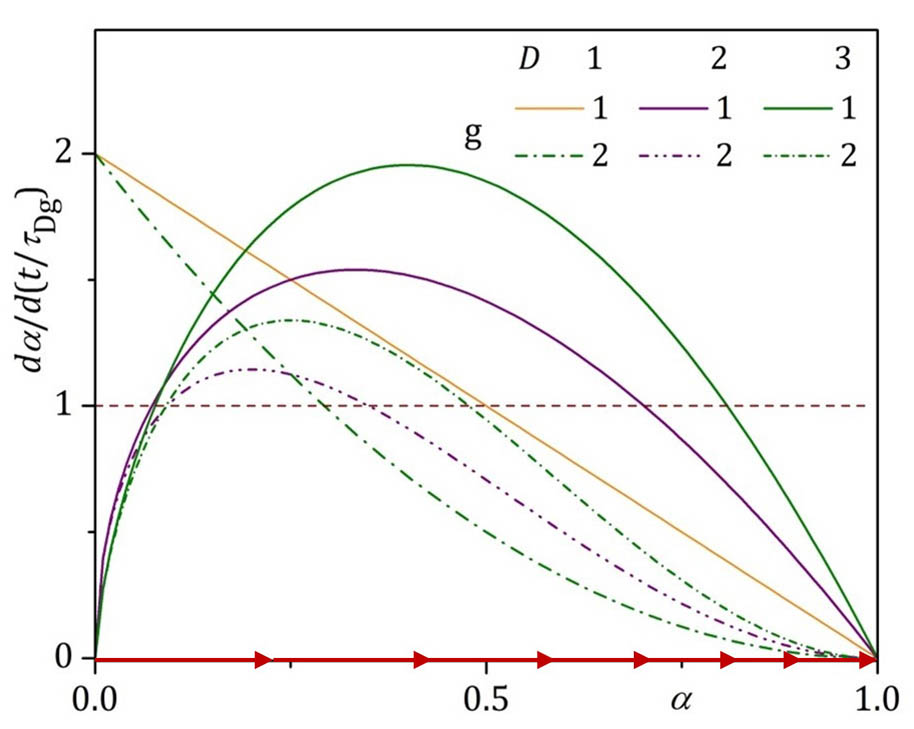
\includegraphics[width=0.9\textwidth]{phase_space.jpg}
	\caption{1D фазово пространство (линия) на модела. Представени са физически важните стойности на параметрите $D$ и $g$.}
	\label{fig:aDg_phase_space}
\end{figure}

Друг важен инструмент за разбирането на поведението на моделите при различен избор на параметрите е фазовата линия (едномерното фазово пространство) представена на фигура \autoref{fig:aDg_phase_space}. От него първото важно наблюдение е, че независимо от избора на параметри $\aDg  = 0 $ и $\aDg = 1$ са двете равновесни точки на системата. Нещо повече - единствената глобално асимптотично устойчива равновесна точка е $\aDg = 1$, докато $\aDg = 0$ е неустойчива. 

Това има последствия за интегрирането - числено и аналитично. Началното условие $\aDg (0) = 0$ се изпълнява и от тривиалното решение $\aDg(t) = 0$, $\forall t > 0$. Този проблем лесно може бъде съобразен и избегнат при аналитичното интегриране на ОДУ. При численото интегриране, което ще правим, за да сме сигурни че ще получим ,,интересното`` решение ще избираме $\aDg = \epsilon$, където $\epsilon > 0$ e ,,малко`` число, близко до машинната грешка (но по-голямо от нея). Тъй като  $\aDg = 1$ е устойчива равновесна точка, грешката от това числено решение ще бъде малка спрямо точното и бихме очаквали да намалява с нарастване на времето (при условие, че численият метод за интегриране има ,,добро`` поведение.

От \autoref{fig:aDg_phase_space} се оправдава и очакването ни за сигмоидния ход на кривите, преди да сме получили решения за ОДУ. Всички модели (без $D=1$) имат инфлексна точка, в която доминиращата обратна връзка се сменя от положителна на отрицателна. Добре се очертава и монотонното намаляване на скоростта при моделите, в които няма положителна обратна връзка ($D=1$). При тях максималната скорост на растеж е била началната, след което процесът само се забавя до ,,достигане`` на равновесие.

\subsection{Получаване на аналитични изрази}
\label{sub:analytic_results}
Разделяме променливите в \autoref{eq:main_aDg_ode} и интегрираме. За простота на записа правим смяната $t \rightarrow t/\tau$. Така получаваме следната имплицитна крива:
\begin{equation}
	\label{eq:integral_aDg_beta_implicit}
	t(\alpha) = \frac{1}{2D}\mathcal{B}\left(\alpha; \frac{1}{D}, 1 - g \right)
\end{equation}
Където $\mathcal{B}\left(x; a, b \right) = \int_{0}^{x} t^{a-1} (1-t)^{b-1} dt$ е непълната не-нормирана бета-функция на Ойлер. Използвайки нейната обратна, можем да запишем формално:
\begin{equation}
	\label{eq:integral_aDg_beta_inverse}
	\alpha(t) = \mathcal{B}^{-1}\left( 2Dt; \frac{1}{D}, 1 - g \right)
\end{equation}
Където съответно $\mathcal{B}^{-1}$ е обратната на бета-функцията. 

Това решение е достатъчно общо, но получаване на затворени изрази за произволни стойности на параметрите $D, g$ в общия случай не е възможно. За целта е разработена и числена процедура, която да интегрира основното ОДУ за произволен избор на параметрите.

Въпреки това, за физически обоснованите, целочислени стойности на параметрите, т.е. $D = 1, 2, 3$ и $g = 1, 2$ е възможно да извършим аналитично интегрирането. За случаите $D + g \le 3$ можем да получим изрази в затворен вид, докато за $D + g > 3$ можем да получим само кривите $t(\alpha)$. Резултатите от интегрирането обобщаваме така:
\begin{align*}
	\noindent\text{За $g = 1:$} \\
	    & \alpha_{11} =  1 - \exp{\left(-2t/\tau_{11}\right)}                                                                                                                                                                                                                                                             \\
	    & \alpha_{21} = \tanh^2 \left(2 t/\tau_{21}\right)                                                                                                                                                                                                                                                                 \\
	    & \frac{t}{\tau _{31}} = \frac{1}{12} \left(\ln \left(\frac{\alpha_{31}^{2/3}+\sqrt[3]{\alpha_{31}}+1}{\left(1-\sqrt[3]{\alpha_{31}}\right){}^2}\right)+2 \sqrt{3}\arctan\left(\frac{\sqrt{3} \sqrt[3]{\alpha_{31}}}{2+\sqrt[3]{\alpha _{31}}}\right)\right) \tag{*}                                               \\
	\noindent\text{За $g = 2:$} \\
	    & \alpha_{12} = \frac{2 t/ t_{12}}{2 t/ t_{12} + 1}                                                                                                                                                                                                                                                                \\
	    & t/\tau_{22} = \frac{1}{4}\left( \frac{\alpha_{22}^{1/2}}{1-\alpha_{22}} + \tanh^{-1} \alpha_{22}^{1/2} \right) \tag{*}                                                                                                                                                                                           \\
	    & \frac{t}{\tau_{32}} = \frac{1}{18} \left(\frac{3 \sqrt[3]{\alpha_{32}}}{1-\alpha_{32}}+\ln \left(\frac{\alpha_{32}^{2/3}+\sqrt[3]{\alpha _{32}}+1}{\left(1-\sqrt[3]{\alpha_{32}}\right){}^2}\right)+2 \sqrt{3}\arctan \left(\frac{\sqrt{3} \sqrt[3]{\alpha_{32}}}{2+\sqrt[3]{\alpha_{32}}}\right)\right) \tag{*} 
\end{align*}
Уравненията, които са отбелязани с $(*)$ не могат да бъдат решени за $\aDg$.
\begin{figure}[H]
	\centering
	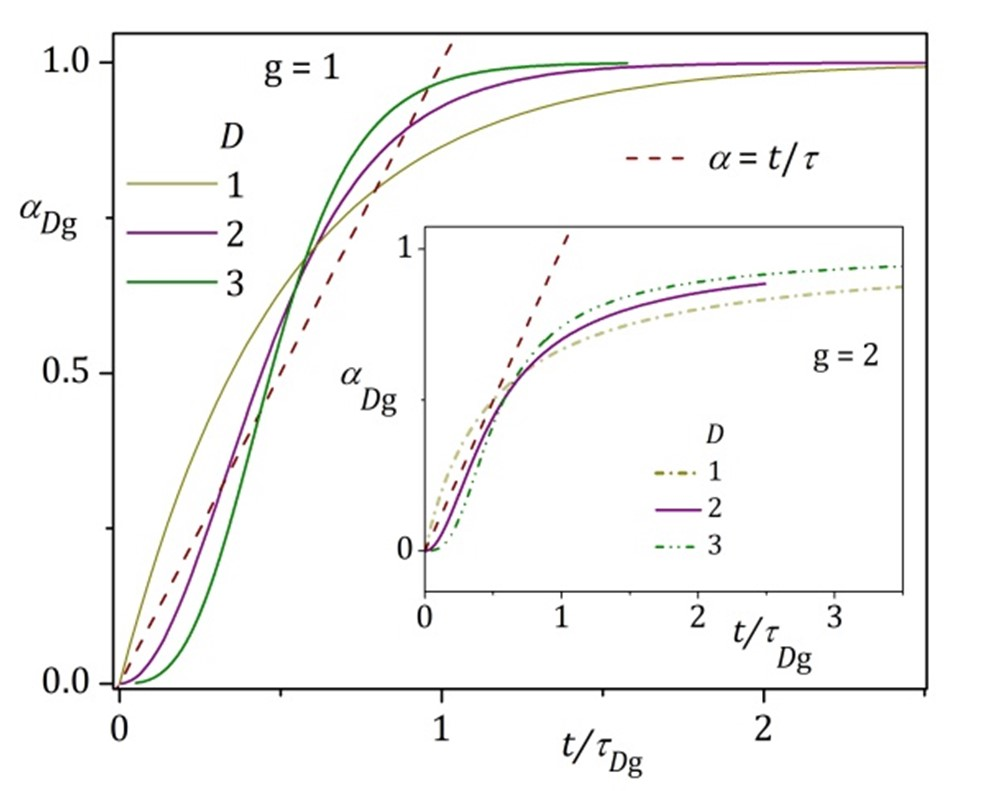
\includegraphics[width=0.9\textwidth]{integral_curves.jpg}
	\caption{Интегрални криви на модела. Основна фигура: $g = 1$, вложена: $g = 2$. Тук правата отговаряща на $\alpha = t/\tau$ е дадена като референтна за по-удобно сравняване на двете фигури.}
	\label{fig:aDg_integral_curves}
\end{figure}

\subsection{Инфлексни точки на модела}
\label{sub:aDg_infl_points}
Както вече беше споменато, в модела имаме два вида обратна връзка - положителна и отрицателна. Точката, в която доминиращата обратна връзка се сменя, е инфлексната точка (когато тя съществува). В този смисъл инфлексната точка е характеристична за режима на кристален растеж, който наблюдаваме и затова получаването на израз за нея като функция на параметрите на модела ще бъде важна задача, която да решим. Необходимо условие за съществуването на инфлексна точка $t^*$ е:
\begin{equation*}
	\alpha'' = \left. \frac{d^2\alpha}{dt^2}\right|_{t = t^*} = 0
\end{equation*}
Диференцираме двете страни на \autoref{eq:main_aDg_ode} по t:
\begin{equation*}
	\alpha'' = -2 \alpha^{-1/D} (1-a)^{g-1}\left[ \left( D g + D - 1 \right)\alpha - D + 1 \right] \alpha'
\end{equation*}
Заместваме $\alpha'$ с дясната страна на \autoref{eq:main_aDg_ode}, групираме членовете по $\alpha$ и получаваме за втората производна:
\begin{equation}
	\label{eq:aDg_second_der}
	\alpha'' = -4 D \alpha^{\frac{D-2}{D}}(1-\alpha)^{2g-1}\left[(D g + D - 1) \alpha - D + 1\right]
\end{equation}
Единствената нула $\alpha^*$ на уравнението $\alpha'' = 0$, която не е една от равновесните точките $\alpha = 0 $ или $\alpha = 1$ e:
\begin{equation}
	\label{eq:aDg_alpha_infl_point}
	\alpha^* = \frac{D - 1}{D g + D - 1}, \qquad D > 1
\end{equation}  
Тъй като в $\alpha_{1g}$ моделите няма положителна обратна връзка, те нямат и инфлексна точка. Това се потвърждава и от монотонно намаляващите криви на \autoref{fig:aDg_phase_space}.
Тук общото решение дадено в \autoref{eq:integral_aDg_beta_implicit} за $t(\alpha)$ ще ни послужи да намерим за кое $t^*$ се достига инфлексната точка $\alpha^*$ (изчисляването на правата непълна ненормирана бета-функция е много по-лесна и добре обусловена числена задача от тази за обратната). Можем да обобщим като кажем, че $\aDg$ моделите имат инфлексна точка в наредените двойки $\{t^*, \alpha^*\}$, такива че:
\begin{equation}
	\label{eq:aDg_tuple_infl_point}
	\left\{t^*; \alpha^* \right\} = \left\{\frac{1}{2D}\mathcal{B}\left( \frac{D - 1}{D g + D - 1}; \frac{1}{D}, 1 - g \right); \frac{D - 1}{D g + D - 1}\right\} 
\end{equation}
Конкретните стойности можем да обобщим в \autoref{tabl:aDg_infl_points}. Интересно наблюдение е, че инфлексните точки са относително ,,рано``, т.е. за ,,малки`` $t, \alpha$, и по-конкретно $\alpha^* < 1/2$ за всеки от наборите параметри. Това е логично, предвид че положителната обратна връзка е ,,по-слаба`` от експоненциалната в модела на Ферхюлст, т.е. процесът на кристален растеж при тези условия се самоограничава относително бързо и  съответно максимумът на скоростта се достига относително рано. Още по-явно се забелязва това в случая на кинетичен контрол, когато $g = 2$. Тогава самоограничаването на процеса е още по-силно.

Интересен факт е, че инфлексните точки са относително ,,близо`` до правата $\alpha = t/\tau$, т.е. използването ѝ като референтна такава на \autoref{fig:aDg_integral_curves} е оправдано за целите на сравняване на хода на кривите.
\begin{table}[htbp]
	\centering
	\caption{Инфлексни точки на $\aDg$ моделите при различни стойности на параметрите $D, g$}
	\label{tabl:aDg_infl_points}
	\resizebox{0.5\textwidth}{!}{%
		\begin{tabular}{@{}cll@{}}
			\toprule
			\multicolumn{1}{l}{D/g} & \multicolumn{1}{c}{1} & \multicolumn{1}{c}{2} \\ \midrule
			1                       & -                     & -                     \\
			2                       & \{0.329; 1/3\}        & \{0.260; 1/5\}        \\
			3                       & \{0.417; 2/5\}        & \{0.365 ; 1/4\}       \\ \bottomrule
		\end{tabular}%
	}
\end{table}
\subsection{Числено интегриране и параметрична идентификация}
\subsubsection{Числено интегриране}
\label{subsub:numeric_integration}
Както беше споменато в \autoref{sub:analytic_results} аналитичното интегриране е трудно за произволни параметри $D, g$. Същевременно ,,обръщането`` на бета-функцията е лошо обусловена числено задача. Причината за това е, че при $\alpha \rightarrow 1$, $t \rightarrow \infty$, т.е. за големи степени на превръщане числените методи за решаване на \autoref{eq:integral_aDg_beta_implicit} ще стават неустойчиви, тъй като задачата е лошо обусловена, независимо от конкретните качества на метода.

От друга страна знаем от \autoref{fig:aDg_phase_space}, че равновесната точка $\alpha = 1$ e устойчива \autoref{eq:main_aDg_ode}. Нещо повече, чрез директно прилагане на правилото за Лайбниц за $n$-та производна на произведение, получаваме че $f^{(n)} (\alpha = 1)  = 0$. Където с $f(\alpha) = 0$ сме означили дясната страна на \autoref{eq:main_aDg_ode}. Т.е. не очакваме да имаме проблеми с устойчивостта на методите.

Директно можем да се възползваме от библиотеката \textit{Scipy} \cite{2020SciPy-NMeth} за програмния език \textit{Python}. \textit{Python} е особено подходящ заради динамичната си типова система, която позволява на функцията \textit{scipy.integrate.solve_ivp()} директно да върне кубичен ермитов сплайн-интерполант на решението в интервала $[t_0, t_{max}]$. 
Единствената особеност тук е, че за да сме сигурни че няма да останем в тривиалното решение $\aDg(t) = 0, \forall t$, ще вземем за начално условие $\aDg(0) = 10^{-10}$.
\begin{minted}{python}
def get_sigmoid(d, g):
    sol = integrate.solve_ivp( # from scipy
        rhs, # 2 * d * ((1 - y) ** g) * (y ** (1 - (1 / d)))
        [SIGMOID_CONFIG["t0"], SIGMOID_CONFIG["t_final"]],
        [SIGMOID_CONFIG["initial_alpha"]],
        args=(d, g),
        dense_output=True,
        method="RK45",
        atol=1e-13,
        rtol=1e-12
    )
    return sol.sol # returns a function object
\end{minted}
Полученият обект е изключително удобен за последваща работа, защото има поведение на функция на един аргумент, която за дадено $t/\tau$ връща стойността на $\alpha$. Конкретната имплементация, която е с по-общ програмен интерфейс може да бъде намерена в скрипта \textit{sigmoid_calculation.py} от \cite{SigmoidToolsGH}.

Резултатите от численото интегриране на $\alpha_{21}$ са показателни за общото поведение на числената процедура и за други избори на параметрите на модела.
\begin{figure}[!ht]
    \centering
    \caption{Числено интегриране до различни $t/\tau$}
        \subfloat[Малки времена]{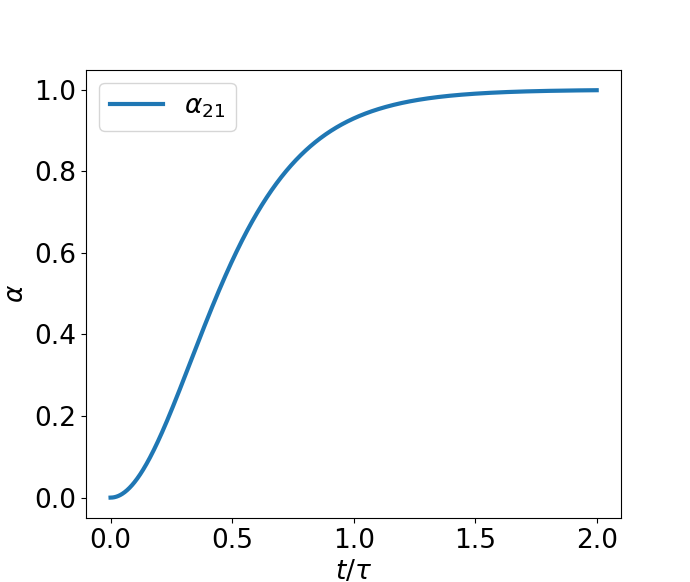
\includegraphics[width=0.47\textwidth]{alpha21_small_tmax.png}}
        \subfloat[Големи времена]{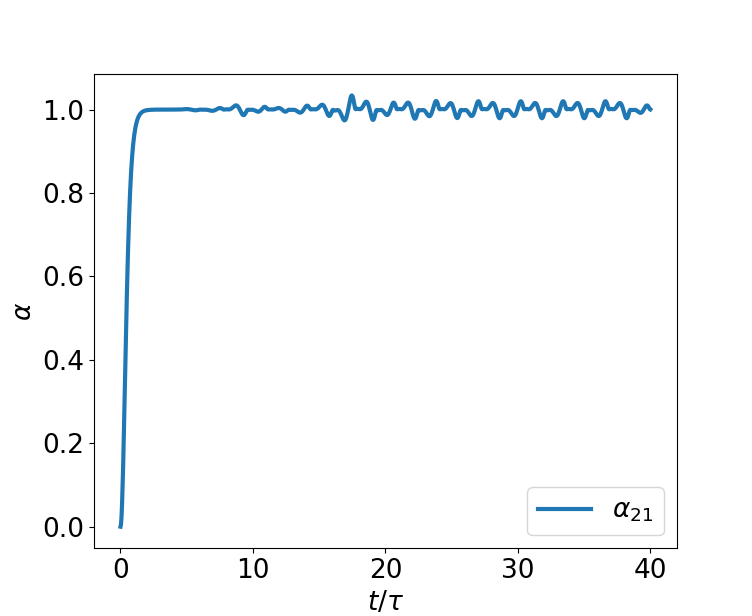
\includegraphics[width=0.48\textwidth]{alpha21_large_tmax.png}}
    \label{fig:a21_numeric}
\end{figure}

\noindent На \autoref{fig:a21_numeric} добре се вижда поведението на числения интегратор. При смяна на метода с такъв с по-сложно поведение (автоматично засичане на неустойчивост и съответен избор на стъпката) резултатите също са аналогични. Резултатът е добър и поведението е ,,хубаво`` за относително широк интервал от времена (в случая на  \autoref{fig:a21_numeric} до около $t_{max}/\tau = 10$, след което численият метод за интегриране става немонотонен. Причината за това е, че $\alpha$ при $t_{max}/\tau = 2$ е на практика достигнало равновесното $\alpha = 1$. От там нататък, разликите на всяка стъпка $\Delta \alpha$ са много малки - от порядъка на машинната грешка $\approx 10^-16$ и това води до наблюдаваното немонотонно поведение.

След числени експерименти за целите на крайната имплементация е избран методът \textit{DOP853} пред \textit{RK45}, тъй като контролът на неустойчивостта  е по-добър и немонотонността се проявява при по-големи $t/\tau$. Използването на методи с адаптивен избор на стъпката ни позволява да интегрираме с малка стъпка само в интервалите, където функцията нараства бързо и да контролираме алгоритъма чрез зададена отнапред относителна грешка.

Този проблем е неизбежен, независимо от метода за интегриране на ОДУ, който използваме но и не е толкова съществен предвид, че експериментите, за които искаме да правим параметрична идентификация на модела, рядко стигат до $\alpha \gg 90\%$. Все пак е важно този ефект да бъде взиман под внимание, когато се разработват оптимизационните методи за намиране на параметрите от експериментални данни, тъй като ,,началото`` на немонотонното поведение - зависи от $D, g, \tau$ и може да се окаже за по-малки $t/\tau$ от представените тук.

Тъй като за $\alpha_{21}$ имаме аналитично решение в затворен вид, можем да изчислим максималната и средната абсолютната грешка за даден интеграционен интервал, например $t/\tau \in [0, 2]$. На \autoref{fig:abs_error_a21} е представена графика на грешката за целия интервал. Очаквано, най-голяма е грешката в инфлексната точка $t/\tau = 0.329$, тъй като там и нарастването на функцията е най-голямо. При направената имплементация максимумът е $8\cdot10^{-9}$, докато средната грешка за интервала е $2\cdot10^{-9}$. 

\begin{figure}[hbtp]
    \centering
    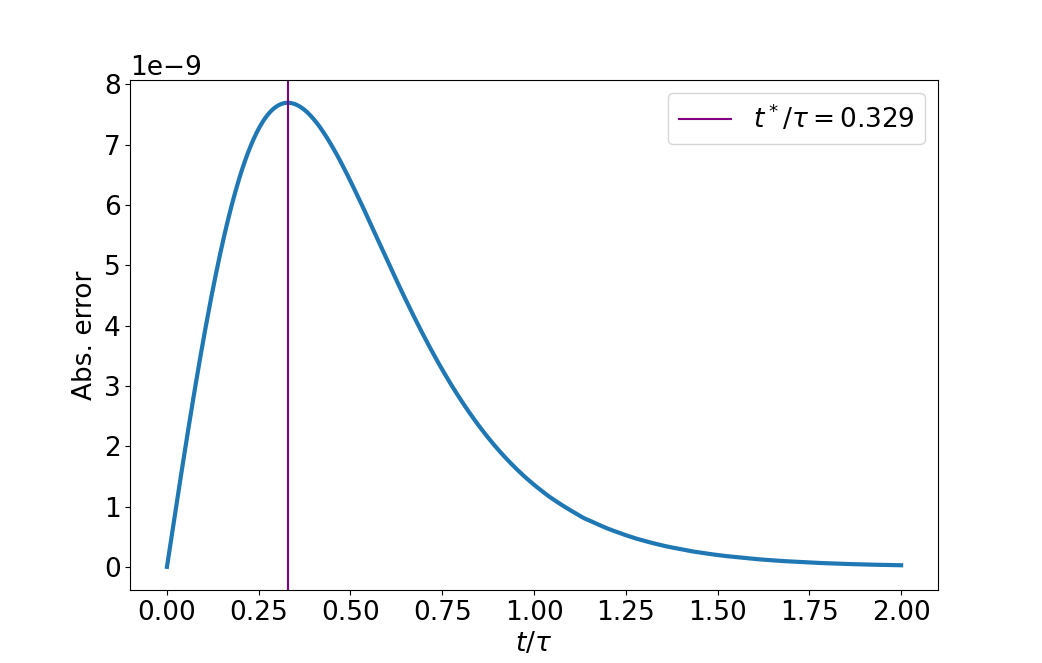
\includegraphics[width=\textwidth]{alpha21_abs_error.png}
    \caption{Абсолютна грешка от численото интегриране за $\alpha_{21}$}
    \label{fig:abs_error_a21}
\end{figure}

\subsubsection{Параметрична идентификация}
\label{subsub:parametric_identification}
Част от целите, които това изследване си поставя, е ,,инструментализацията`` на разработения модел, т.е. разработка на обща процедура, която да позволява от експериментални данни (реални или от числен експеримент) да се определят $D$ (дали растящият кристал e едно, дву - или тримерен) и $g$ (дифузионен или кинетичен контрол). 

Допълнително от \autoref{eq:time_scale} е ясно, че времевата скала $\tau$ съдържа началната скорост $r_0(g)$, която пък съдържа температурната зависимост на процеса. Затова определянето и на $\tau$ с останалите два параметъра ще бъде част от процедурата за параметрична идентификация. За целта умножаваме двете страни на \autoref{eq:main_aDg_ode} с $\tau$ и ще работим с тази ,,полу-обезразмерена`` форма на основното ОДУ.

Следващите процедури надграждат над тези от \autoref{subsub:numeric_integration}, тъй като дясната страна на основното ОДУ е непрекъсната по параметрите $D, g, \tau$. Това позволява да работим със стандартни подходи за параметрична идентификация за непрекъснати функции и по тази причина резултатите от оптимизацията ще са реални числа, а не цели. 

Тъй като ние целим да запазим физичния смисъл на параметрите $D, g$ резултатите от оптимизацията ще служат само за насока за режима на растеж и избор на правилната крива от \autoref{sub:analytic_results}. Параметри получени от оптимизацията, които не отговарят на предположенията поставени при извеждането ще разглеждаме като невъзможност на модела да обясни конкретния експеримент. 

За целите на следващите два параграфа ще въведем следната дефиниция:
\begin{definition}{Вектор на остатъците}{resd_vector}
    Ще предполагаме, че имаме $N$ експериментални точки $(t^{i}, \alpha^i)$ за $i = 1,...,N$. Ще отбележим с $\alpha_{D,g,\tau}^i$ стойността на $\alpha_{D,g,\tau}(t^i)$ при конкретен избор на параметрите $D, g, \tau$. Векторът на остатъците $\varepsilon$ тогава дефинираме като:
    \begin{equation*}
        \label{eq:resd_vector}
        \varepsilon(D, g, \tau) = \left( \alpha^1 - \alpha_{D,g,\tau}^1, \alpha^2 - \alpha_{D,g,\tau}^2,  ..., \alpha^N - \alpha_{D,g,\tau}^N \right)
    \end{equation*}
\end{definition}
\noindent Тогава общата оптимизационна задача, която ще решаваме е:
\begin{equation}
    \label{eq:optmiz_problem}
    (D^*, g^*, \tau^*) = argmin_{(D, g, \tau)} \lVert \varepsilon(D, g, \tau) \rVert
\end{equation}

\paragraph{Нелинейни най-малки квадрати (NLSQ)} Тук нормата, с която определяме големината на вектора на остатъците е втората норма $\lVert \cdot \rVert_{2}$:
\begin{equation*}
    \lVert  \varepsilon \rVert_{2} = \sqrt{\sum_{i} | \varepsilon_i| ^ 2}
\end{equation*}
Така получаваме класическата задача за нелинейни най-малки квадрати. Тъй като това е достатъчно добре изучена задача и броят експериментални точки е малък ($<20$) особено подходящ е алгоритъмът на \textit{Levenberg-Marquard} като модификация на алгоритъма на \textit{Gauss-Newton} с доверителна област. \cite{Kelley1999} 

Имплементация на \textit{Levenberg-Marquard} може да бъде намерена в пакета \textit{MIN\-PACK} за \textit{Fortran} \cite{MinpackGH}. Тази импле\-мен\-та\-ция е доказано ,,добра`` и ши\-ро\-ко\-изпол\-звана с различни опции като пресмятане на матрицата на Якоби чрез алгоритмично диференциране. Особено удобно е, че модулът \textit{Optimize} от \textit{SciPy} предоставя програмен интерфейс за \textit{Python} към \textit{MINPACK} \cite{2020SciPy-NMeth}. Този интерфейс се нуждае единствено от функцията, която пресмята вектора на остатъците $\varepsilon(D,g,\tau)$, начално предположение за стойността на параметрите и по желание на потребителя - експлицитни граници за параметрите и доверителната област.

Най-общо функцията за параметрична идентификация за произволен списък от експериментални точки $(t^{i}, \alpha^i)$ изглежда така:
\begin{minted}{python}
def fit_data(dat):
    fit = optimize.least_squares( # from the scipy module optimize
        lsq_cost, # function that calculates resds vec for given params
        x0=[
            FINDER_CONFIG["d_ini"],
            FINDER_CONFIG["g_ini"],
            FINDER_CONFIG["tau_ini"],
        ],
        args=(dat,),
        verbose=2,
        bounds=(
            (
                FINDER_CONFIG["d_min"],
                FINDER_CONFIG["g_min"],
                FINDER_CONFIG["tau_min"],
            ),
            (
                FINDER_CONFIG["d_max"],
                FINDER_CONFIG["g_max"],
                FINDER_CONFIG["tau_max"],
            ),
        ),
    )
    d = fit.x[0]
    g = fit.x[1]
    tau = fit.x[2]
    return fit, d, g, tau
\end{minted}

Конкретната имплементация с допълнително филтриране на данни, които са извън интеграционния интервал (с цел избягването на екстраполация) и команден интерфейс за работа с \textit{.csv}-файлове може да бъде намерена в скрипта \textit{parameter_finder.py} от \cite{SigmoidToolsGH}.

\paragraph{Равномерно приближение (uniform/minimax)} Тук искаме да минимизираме безкрайност нормата на вектора на остатъците $\lVert \cdot \rVert_{\infty}$:
\begin{equation*}
    \lVert \varepsilon \rVert_{\infty} = \max_{i} | \varepsilon_i| 
\end{equation*}
От общата теория е известно, че безкрайност нормата не е непрекъснато диференцируема и съответно градиентни методи за минимизирането ѝ не са подходящи. Не съществува и обобщен алгоритъм като \textit{Levenberg-Marquard} за решаването на тази задача.

Въпреки тези проблеми, намирането на най-доброто равномерно приближение е интересно практически, защото гарантира, че за дадени параметри на модела, максималната грешка не надвишава определена стойност.

За да намерим минимума на тази норма ще използваме модификация на Монте Карло метода на Метрополис, т.нар. \textit{симулирано закаляване}. Общият алгоритъм е много прост \cite{wiki:Simulated_annealing} и е необходимо целевата функция да е само $C^0$-непрекъсната:
\begin{algorithm}
\caption{Симулирано закаляване}\label{alg:cap}
    \begin{algorithmic}[1]
    \State $p \gets p_0$ \Comment{Начално предположение}
    \While{$k < k_{max}$} \Comment{Максимален брой итерации $k_{max}$}
        \State $T \gets Temperature (k)$
        \State $p_{new} \gets Neighbour(p)$
        \If{$\mathcal{P}\left(E(p), E(p_{new}), T\right) \ge RandomUniform(0,1)$}
            \State $p \gets p_{new}$
        \EndIf
    \EndWhile
    \State $ \text{\textbf{output}}~~p$
    \end{algorithmic}
\end{algorithm}

За конкретната имплементация е необходимо да бъдат дефинирани: началния вектор от параметри $p_0$, целевата функция $E(p
)$, функция с която да избираме следващия кандидат: $Neighbour(p)$, как понижаваме температурата на стъпка $k$ - $Temperature (k)$ и дискриминативна функция $\mathcal{P}\left(E(p), E(p_{new}), T\right)$, спрямо която решаваме дали запазваме новите параметри (напр. Болцманово разпределение в класическия алгоритъм на Метрополис). За симулирането закаляване можем да обобщим следното:
\begin{itemize}
    \item Това е глобална оптимизационна процедура.
    \item Стохастичен (случаен) метод.
    \item Успешността на алгоритъма \textit{силно} зависи от изброените по-горе функции.
\end{itemize}
Поради тези особености, съществуват разработени множество конкретни реализации - различни енергетични разпределения, рестартиране на алгоритъма, множество различни стартове комбинирани с локално търсене и т.н.  \cite{Xiang1997} \cite{Xiang2013}
В \textit{SciPy} модула \textit{Optimize} е направена имплементация на симулирано закаляване под името \textit{scipy.optimize.dual_annealing()} на база \cite{Xiang2013}, където за $Neighbour(p)$ е избрано например разпределението на Коши-Лоренц. Крайният интерфейс се нуждае единствено от целева функция, начално предположение и граници за всеки от параметрите. Допълнителни опции като избор на максималния брой итерации $k_{max}$ също са налични.

Най-общо функцията за параметрична идентификация за произволен списък от експериментални точки $(t^{i}, \alpha^i)$ изглежда така:
\begin{minted}{python}
def fit_data(dat):
    fit = optimize.dual_annealing(uniform_cost,
    x0 = (FINDER_CONFIG["d_ini"], 
    FINDER_CONFIG["g_ini"], 
    FINDER_CONFIG["tau_ini"]
    ), 
    bounds=((FINDER_CONFIG["d_min"], FINDER_CONFIG["d_max"]), 
            (FINDER_CONFIG["g_min"], FINDER_CONFIG["g_max"]),
            (FINDER_CONFIG["tau_min"], FINDER_CONFIG["tau_max"])),
    args=(dat,),
    )

    d = fit.x[0]
    g = fit.x[1]
    tau = fit.x[2]
    return fit, d, g, tau
\end{minted}
Командния интерфейс за работа с \textit{.csv}-файлове може да бъде намерен в скрипта \textit{parameter_finder_uniform.py} от \cite{SigmoidToolsGH}.
\subsection{Верификация на модела спрямо JMAKn}
Моделът $\aDg$ има за цел да бъде физически осмислена в контекста на кристализация из разтвор алтернатива на JMAKn, затова ще направим подробно сравнение на двата модела и ,,верификация`` на  $\aDg$ спрямо JMAKn.
С цел последващото изложение и по-директна аналогия, ще запишем JMAKn във вида:
\begin{equation}
    \label{eq:jmakn_with_time_scale}
    \alpha(t) = 1 - \exp{\left[ - \left( \frac{2 t}{\tau_{JMAKn}} \right)^n \right]}
\end{equation}
Т.е. сме заместили в \autoref{eq:jmak}: $k = (2/\tau_{JMAKn})^n$, тъй като $\tau_{JMAKn}$ може да бъде толкова произволно колкото $k$ не сме променили общността на записа.
\subsubsection{Диференциална форма на JMAKn}
В литературата рядко може да бъде намерена диференциалната форма на JMAKn или ако е публикувана, то нейното извеждане не директно направено \cite{Avramov2005}. За целта ние ще започнем като получим скоростта на нарастване на степента на трансформация $d \alpha/d t$ за JMAKn. Първо решаваме \autoref{eq:jmakn_with_time_scale} за $t/\tau_{JMAKn}$:
\begin{equation*}
    t/\tau_{JMAKn} = \frac{1}{2}\left[ - \ln{\left( 1- \alpha \right)} \right]^{1/n}
\end{equation*}
и диференцираме по $\alpha$:
\begin{equation*}
    \frac{d \left( t/\tau_{JMAKn} \right) }{d \alpha} = \frac{\left[ - \ln{\left( 1- \alpha \right)} \right]^{\frac{1-n}{n}}}{2n(1-\alpha)}
\end{equation*}
заедно с теоремата за производна на обратната функция, получаваме:
\begin{equation}
    \label{eq:jmak_differential_form}
    \frac{d \alpha}{d (t/\tau_{JMAKn})} = 2n(1-\alpha)\left[ \ln{\left( \frac{1}{1-\alpha} \right)} \right] ^ {\frac{n-1}{n}}
\end{equation}
Дясната страна на това ОДУ за $n = 2$ може да бъде намерено формулирано като вероятностно разпределение за $\alpha$ в \cite{Stoyanov1988} \cite{Fanfoni1998}.

От този запис веднага се вижда съответствието с \autoref{eq:main_aDg_ode}. За $n = 1$ дясната страна изцяло съвпада с тази на $\alpha_{11}$, както и интегралната крива от \autoref{eq:jmak_time_scale} и тази за $\alpha_{11}$ от \autoref{sub:analytic_results}.

\noindent Нещо повече, нека вземем предвид следния ред на Тейлър развит около $\alpha = 0$:
\begin{equation}
    \ln{\left( \frac{1}{1-\alpha} \right)} = \sum_{k=1}^\infty \frac{\alpha^k}{k}, \qquad |\alpha| < 1
\end{equation}
И развием логаритъма в скобите от \autoref{eq:jmak_differential_form} взимайки само линейният член ($k=1$), получаваме:
\begin{equation}
    \label{eq:jmakn_power_series}
    \frac{d \alpha}{d \left( t/\tau_{JMAK} \right)} = 2 n \alpha^{\frac{n-1}{n}}\left(1-\alpha\right) + O(\alpha^{^{\frac{2(n-1)}{n}}})
\end{equation} %% TODO: check power
Тогава за \textbf{малки} степени на превръщане ($\alpha \approx 0$): $\aDg$ и JMAKn съвпадат с $D = n$, $g = 1$ и $\tau_{JMAKn} = \tau_{D1}$.

\subsubsection{Инфлексни точки на JMAKn}
В литературата е разпространена $\left\{t^*/\tau_{JMAKn};\alpha^* \right\} = \left\{1/2; 1 - 1/e \right\}$ \cite{Avramov2005} като единствена инфлексна точка на JMAKn, която не зависи от избора на $n$. Това очевидно няма как да бъде вярно, особено предвид че при $n = 1$ такава инфлексна точка не съществува (отново има само отрицателна обратна връзка).
Следвайки процедурата в \autoref{sub:aDg_infl_points} можем аналогично да получим за инфлексната точка на JMAKn при конкретен избор на $n$:
\begin{equation}
    \label{eq:jmak_infl_point}
     \left\{ t^* / \tau_{JMAKn}; \alpha^* \right\}  = \left\{\frac{1}{2} \left( \frac{n-1}{n} \right); 1-e^{\frac{1}{n} - 1}\right\}
\end{equation}
Ако в \autoref{eq:jmak_infl_point} пуснем $n \rightarrow \infty$ в дясната страна ще получим именно $\left\{1/2; 1 - 1/e \right\}$.
Можем и да изключим $n$, за да получим директно имплицитна крива за $\alpha^*$ свързваща двете координати на инфлексната точка:
\begin{equation*}
    t^*/\tau_{JMAKn} (\alpha ^ *) = \frac{1}{2}\left( \ln{\left( \frac{1}{1-\alpha^*} \right)} \right)^{1+\ln{(1-\alpha^*)}}, \qquad 0 < \alpha^* \le  1 - 1/e 
\end{equation*}
В \autoref{tabl:jmak_infl_points} са представени обобщено инфлексните точки за избрани стойности на $n$, които могат да бъдат срещнати често в литературата. Допълнително на \autoref{fig:infl_points_curves} са представени параметричните криви, даващи инфлексните точки на JMAKn, $\alpha_{D1}$  и $\alpha_{D2}$ при вариране на $D$ или $n$. Кривата за \textcolor{green}{JMAKn} е винаги над правата $\alpha^* = t^*$, докато $\aDg$ я пресичат. Трябва да се има предвид, че с тези криви следва да се работи внимателно, защото за дадена точка от тях не е директно очевидно на каква стойност на параметрите отговаря. От друга страна те могат да служат за ориентир за ,,близостта`` на моделите при тези различни параметри - например се вижда, че $\alpha_{21}$ e най-близо до JMAKn за $n = 1.725$, вместо $n = 2$.

\begin{table}[hbpt]
\centering
\resizebox{\textwidth}{!}{%
\begin{tabular}{ccccccc}
\hline
\textbf{n}                                     & \textbf{1} & \textbf{1.725}    & \textbf{2}         & \textbf{2.43}     & \textbf{3}        & \textbf{4}        \\ \hline
$\left\{(t^*/\tau_{JMAK_n}); \alpha^*\right\}$ & -          & $\{0.303;0.343\}$ & $\{0.354; 0.393\}$ & $\{0.402;0.445\}$ & $\{0.437;0.487\}$ & $\{0.465;0.528\}$ \\ \hline
\end{tabular}%
}
\caption{Инфлексни точки на JMAKn при различни стойности на $n$}
\label{tabl:jmak_infl_points}
\end{table}
\begin{figure}[hbtp]
    \centering
    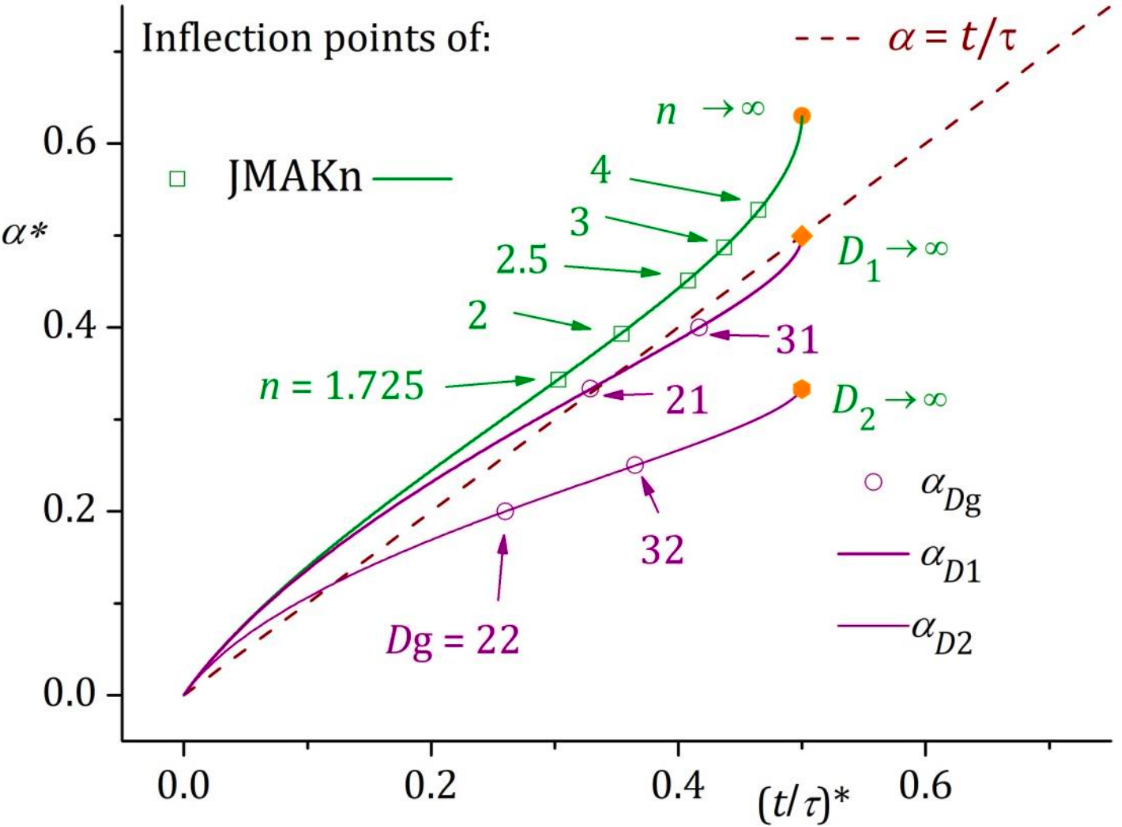
\includegraphics[width=0.80\textwidth]{adg_jmakn_infl_points.png}
    \caption{Инфлексни точки на JMAKn и $\aDg$ при различни стойности на параметрите}
    \label{fig:infl_points_curves}
\end{figure}
\subsubsection{Числено сравнение (фитване) на JMAKn и \texorpdfstring{$\aDg$}{αDg}}
Тук ще използваме процедурите разработени в \autoref{subsub:parametric_identification} за да намерим кои параметри на $\aDg$ водят до крива най-близо (метрично) до $JMAKn$ за дадено $n$ и обратно - кой избор на $n$ води до JMAKn крива най-близо до $\alpha_{D1}$ за дадено $D$.
\autoref{eq:jmakn_power_series} показва, че двата модела са близки за малки $\alpha$ при съответен избор на параметрите, затова в този параграф ще генерираме гъста мрежа от точки ($\Delta t < 0.001$) и стойности, така че $\alpha \in [0, 0.999]$ от единия модел и ще го ,,фитнем`` с другия с \textit{NLSQ} (JMAKn и $\aDg$) и \textit{Uniform} (JMAKn). Тъй като $\alpha_{11}$ съвпада аналитично с JMAK1, най-интересни ще са ни стойностите за  $D \ge 2$.  По този начин ще получим представа в по-широк интервал как биха и до колко си съответстват двата модела.  

Като начало въвеждаме безразмерен конверсионен фактор между двете скали, за да можем по-удобно да покажем разликата между тях. Можем и да въведем по-сложна зависимост между скалите, но това трудно би било оправдано, предвид че за малки $\alpha$ двете трябва да съвпадат точно.
\begin{equation*}
    \tau_{JMAKn} = c_{f} \tau_{Dg}
\end{equation*}

\paragraph{Фитване на $\aDg$ с JMAKn}
Ще започнем като намерим за $\alpha_{21}$ и $\alpha_{31}$ по NLSQ кое е това $n$, за което е най-близка съответната JMAKn-крива. На \autoref{fig:fit_adg_with_jmakn} са представени тези резултати. За конверсионния фактор получаваме $c_{f} \approx 1.1$. Т.е. дори в този широк интервал двете времеви скали са относително близки. Разликите са по-скоро в $D$ и $n$, които са значими, особено предвид че това са експоненти в изразите.
\begin{figure}[hbpt]
    \centering
    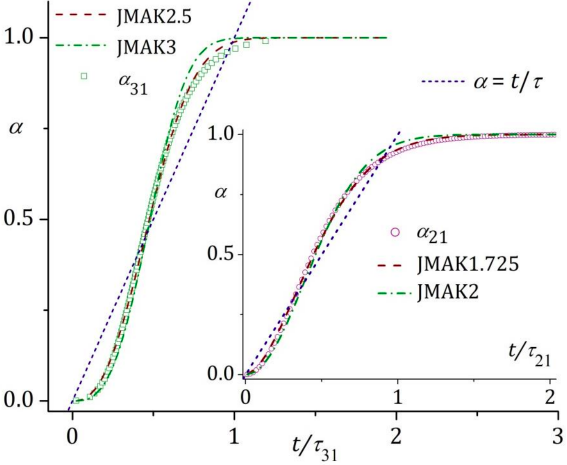
\includegraphics[width=0.8\textwidth]{alpha21andalpha31vsjmak.png}
    \caption{Фитване на $\alpha_{31}$ (основна фигура) с JMAK2.5 и $\alpha_{21}$ с JMAK1.725 (вложена)}
    \label{fig:fit_adg_with_jmakn}
\end{figure}
Същите две графики ще представим и в т.нар. Аврами координати (двойно логаритмични), в които моделът JMAKn се линеаризира. Тези координати са били исторически важни за параметрична идентификация на модела, тъй като тогава не е необходимо да се решава задачата за нелинейни най-малки квадрати. \cite{Fanfoni1998} Линеаризацията изглежда така: 
\begin{equation*}
    \ln{\ln{\left(\frac{1}{1-\alpha}\right)}} = \ln{\left(\frac{t}{\tau_{JMAKn}}\right)}
\end{equation*}
\begin{figure}[!ht]
    \centering
        \caption{Фитване на $\aDg$ с JMAKn в Аврами координати}
        \subfloat[$\alpha_{21}$]{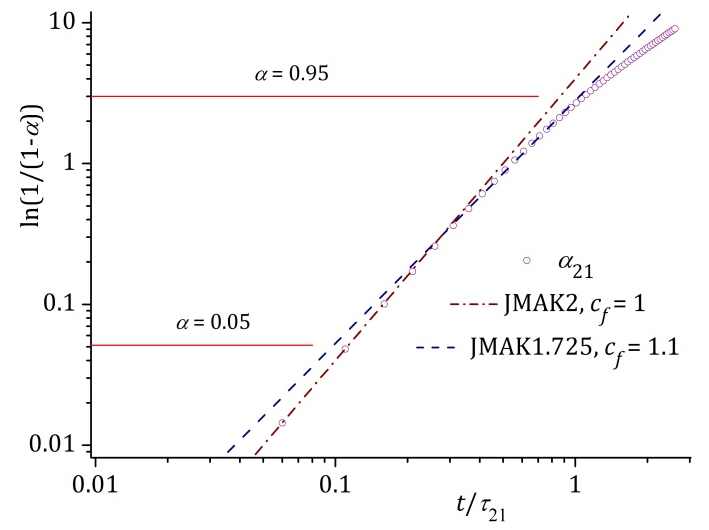
\includegraphics[width=0.48\textwidth]{avramia21.png}}
        \subfloat[$\alpha_{31}$]{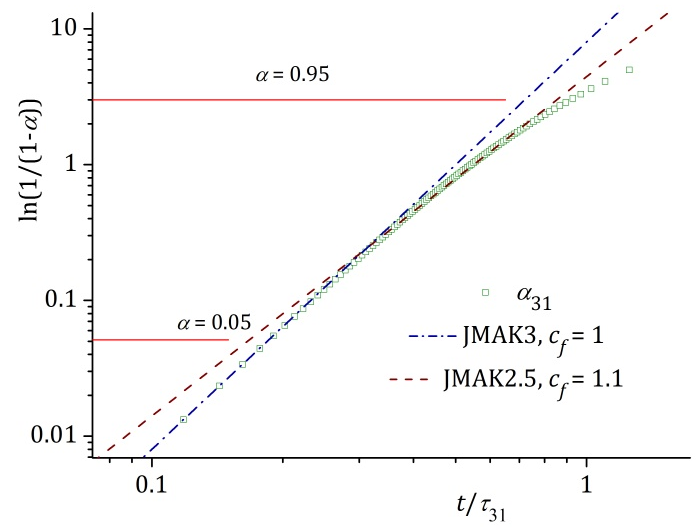
\includegraphics[width=0.48\textwidth]{avramia31.png}}
    \label{fig:avrami_coords_adg_jmak}
\end{figure}
Да обърнем внимание, че в Аврами координати заради нелинейността на осите, малки отклонения всъщност могат да са значителни в линейни координати. Интересен е и ,,десният завой`` на $\aDg$ моделите от JMAKn при големи степени на трансформация.
\begin{figure}[!ht]
    \centering
        \caption{Фитване на $\aDg$ с JMAKn за различни стойности на $\alpha_{upper}$}
        \subfloat[$\alpha_{21}$]{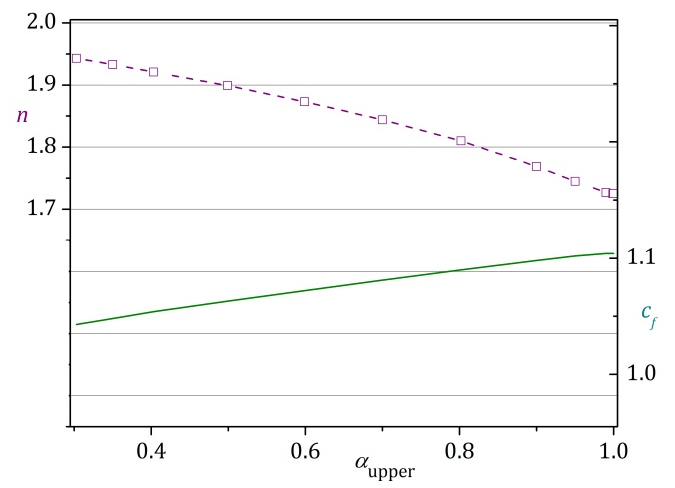
\includegraphics[width=0.48\textwidth]{avramia21_jmak_alphamax_change.png}}
        \subfloat[$\alpha_{31}$]{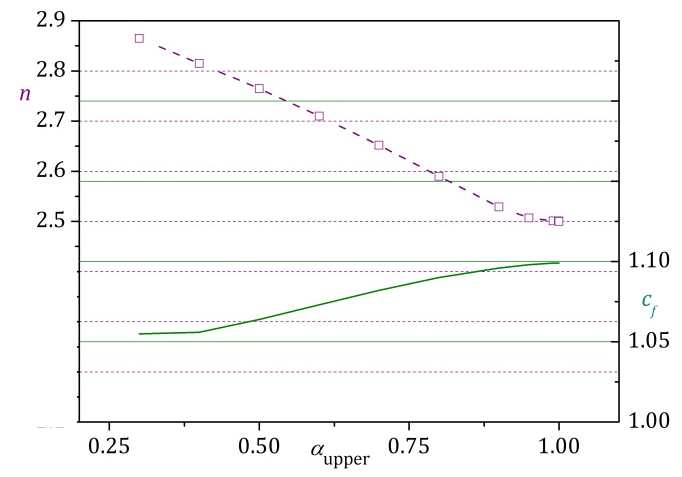
\includegraphics[width=0.49\textwidth]{avramia31_jmak_alphamax_change.png}}
    \label{fig:avrami_coords_adg_jmak_moving_alpha_max}
\end{figure}

На \autoref{fig:avrami_coords_adg_jmak_moving_alpha_max} са комбинирани идеите до тук, като са проведени параметрични идентификации. Данните генерирани от $\aDg$, са такива че $\alpha \in [0, \alpha_{upper}]$, като пък $\alpha_{upper} \in [0.1, 0.999]$. Така се вижда добре нарастването на разликата между $D$ и $n$, съответно и промяната на $c_{f}$ от $1$ до $\approx 1.1$.

От настоящия параграф и фигурите се очертава ясна картина - резултатите от параметричната идентификация зависят от размаха на данните по $\alpha$. Това означава, че трябва внимателно да боравим с експериментални измервания за степента на превръщане, особено когато процесът не е доведен докрай, тъй като тази зависимост от $\alpha_{upper}$ може да скрие ,,истинския`` модел описващ данните. 
%% TODO: interpolate
Глобално оптималните параметри ($\alpha_{upper} \approx 1$) водят до крива, която е метрично близка (в $\lVert \cdot \rVert_{2}$-норма) до съответната $\aDg$, но не я интерполира в $\alpha \rightarrow 0$. Обратно, развитието в ред на Тейлър от \autoref{eq:jmakn_power_series} е много близо до $\aDg$-кривата в началото, но разликата нараства значително с нарастване на $\alpha$.
\paragraph{Фитване на JMAKn с $\aDg$} Ще използваме процедурите разработени в \autoref{subsub:parametric_identification} за да направим параметрична идентификация за данни генерирани от JMAKn при $\alpha \in [0, 0.9999]$. Ще фиксираме $g = 1$ и ще оставим само $D$ и $c_{f}$ да получим като резултат от оптимизацията. Получените параметри са обобщени в \autoref{tabl:fit_jmak_with_adg}.
\begin{table}[hbtp]
\centering
\resizebox{0.7\textwidth}{!}{%
\begin{tabular}{@{}ccccc@{}}
\toprule
\textbf{n от JMAKn}            & \textbf{D}                    & $\boldsymbol{c_{f}}$               & $\boldsymbol{R^2}$                     & \textbf{Процедура}              \\ \midrule
                                 & 1.002                         & 1.00026                        & 0.9999992                          & NLSQ                            \\
\multirow{-2}{*}{\textbf{1}}     & \cellcolor[HTML]{EFEFEF}1     & \cellcolor[HTML]{EFEFEF}0.9999 & \cellcolor[HTML]{EFEFEF}0.99999998 & \cellcolor[HTML]{EFEFEF}UNIFORM \\
                                 & 1.989                         & 1.104                          & 0.9994                             & NLSQ                            \\
\multirow{-2}{*}{\textbf{1.725}} & \cellcolor[HTML]{EFEFEF}1.966 & \cellcolor[HTML]{EFEFEF}1.105  & \cellcolor[HTML]{EFEFEF}0.9993     & \cellcolor[HTML]{EFEFEF}UNIFORM \\
                                 & 2.371                         & 1.109                          & 0.9991                             & NLSQ                            \\
\multirow{-2}{*}{\textbf{2}}     & \cellcolor[HTML]{EFEFEF}2.352 & \cellcolor[HTML]{EFEFEF}1.110  & \cellcolor[HTML]{EFEFEF}0.9991     & \cellcolor[HTML]{EFEFEF}UNIFORM \\
                                 & 2.993                         & 1.105                          & 0.99883                            & NLSQ                            \\
\multirow{-2}{*}{\textbf{2.43}}  & \cellcolor[HTML]{EFEFEF}3.000 & \cellcolor[HTML]{EFEFEF}1.108  & \cellcolor[HTML]{EFEFEF}0.99882    & \cellcolor[HTML]{EFEFEF}UNIFORM \\
                                 & 3.073                         & 1.106                          & 0.99879                            & NLSQ                            \\
\multirow{-2}{*}{\textbf{2.5}}   & \cellcolor[HTML]{EFEFEF}3.036 & \cellcolor[HTML]{EFEFEF}1.107  & \cellcolor[HTML]{EFEFEF}0.99884    & \cellcolor[HTML]{EFEFEF}UNIFORM \\ \midrule
                                 & 3.794                         & 1.100                          & 0.99859                            & NLSQ                            \\
\multirow{-2}{*}{\textbf{3}}     & \cellcolor[HTML]{EFEFEF}3.801 & \cellcolor[HTML]{EFEFEF}1.102  & \cellcolor[HTML]{EFEFEF}0.99857    & \cellcolor[HTML]{EFEFEF}UNIFORM \\
                                 & 5.215                         & 1.083                          & 0.99828                            & NLSQ                            \\
\multirow{-2}{*}{\textbf{4}}     & \cellcolor[HTML]{EFEFEF}5.267 & \cellcolor[HTML]{EFEFEF}1.084  & \cellcolor[HTML]{EFEFEF}0.99829    & \cellcolor[HTML]{EFEFEF}UNIFORM \\ \bottomrule
\end{tabular}%
}
\caption{Резултати от фитването на JMAKn с $\aDg$ при фиксирано $g = 1$}
\label{tabl:fit_jmak_with_adg}
\end{table}

Двете задачи за най-малки квадрати не са напълно еквивалентни (от JMAKn да намерим параметрите на $\aDg$ и обратно). Близките резултати и в двата случая, показват че в най-общ смисъл $n = 1.725$ съответства на $D = 2$ и $n = 3$ на $D = 2.43$ за достатъчно голям размах на данните по степента на трансформация $\alpha$. Факторът $c_{f}$ и в двата случая е консистентно $\approx 1.1$. Така очертаваме съответствие между параметрите на двата модела, което ще е удобно за рационализиране на експериментални данни описани в литературата с JMAKn. 

За да обобщим казаното в този параграф можем да построим графика $n vs. D$ в интервала $2 \le D \le 3$. От \autoref{fig:nvsd_graph} се вижда, че тази зависимост е линейна. 
\begin{figure}[hbpt]
    \centering
    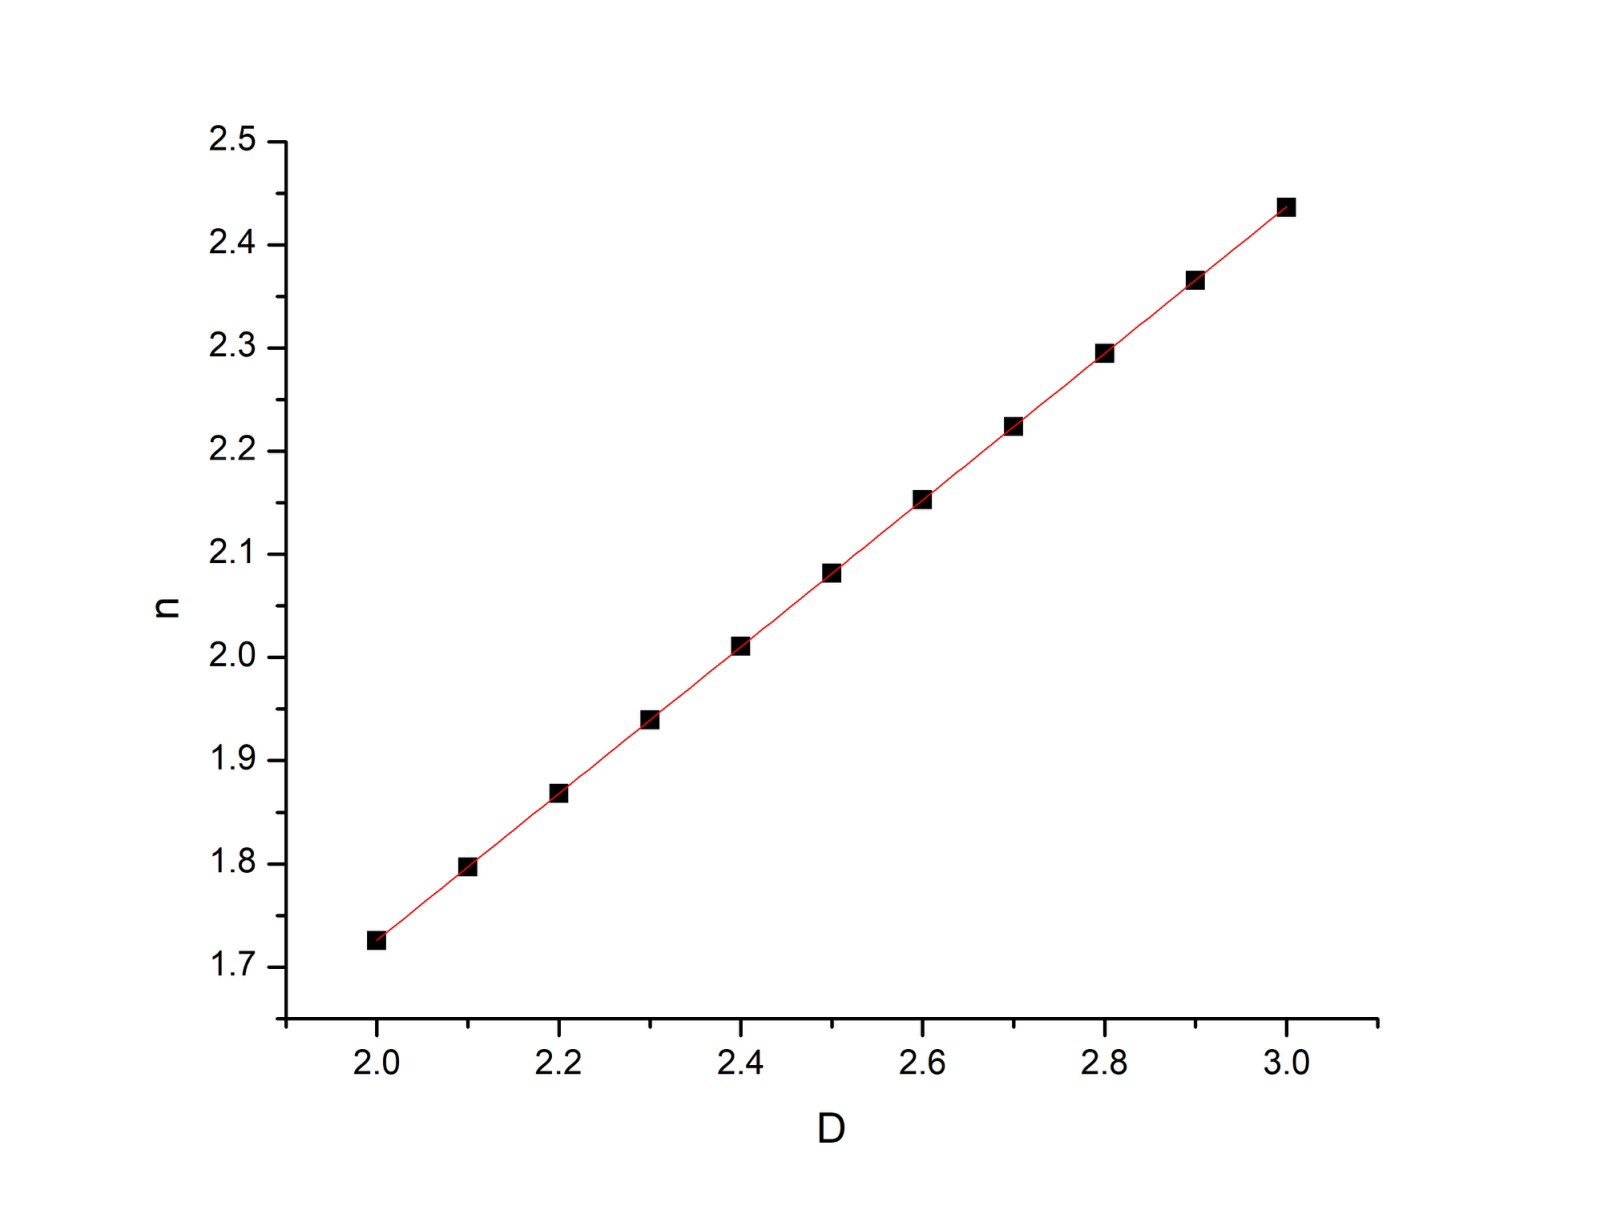
\includegraphics[width=\textwidth]{nvsd.png}
    \caption{Графика на съответствието между $D$ от $\aDg$ и $n$ от най-доброто метрично приближение с JMAKn. Уравнението на правата е $n  = 0.30385 D + 0.71106$} с коефициент на корелация: $R^2 \approx 1 - 1.31 \cdot 10^{-6}$.
    \label{fig:nvsd_graph}
\end{figure}
Като се замести $D = 1$ в уравнението на правата (екстраполация назад) от \autoref{fig:nvsd_graph} се получава $n = 1.01491$, което не е твърде голяма грешка спрямо истинската стойност, предвид че екстраполираме. В този смисъл това уравнение на права може да бъде полезен инструмент за ,,конверсия`` между двата модела.
\subsection{Валидиране с експериментални данни}
\label{sub:experimental_validation}
Основната цел, която си поставихме с този модел е да дадем алтернатива на JMAKn, чиито параметри да носят физически смисъл за целите на изотермична кристализация из разтвор. За да покажем, че това е така ще направим валидиране с реални експериментални данни.
За целите на тази секция ще се фокусираме върху експериментните проведени от \textit{Min, Sinclair, et. al.} \cite{Min2005}.  В  това изследване е използвана тунелна електронна микроскопия (ТЕМ) за изследване на кинетиката на кристализация на тънки $Ta_2O_5$-филми (стъкла) отлагани върху силициеви субстрати. Изследванията са проведени за три различни температури - $790^\circ~C, 820^\circ~C, 850^\circ~C$. Кристализацията при този експеримент е квази-двумерна (2D), тъй като самите тънки филми могат да се разглеждат като квази-двумерни обекти. За трите различни температури са получени стойности за $n$ в JMAKn съответно $n = 2.5, 1.9, 1.7$. Това означава, че няма как използвайки получените скали всички данни да бъдат прескалирани, така че да бъдат описани от една крива.

За да покажем предимствата на $\aDg$ ще използваме $\alpha_{21} = \tanh^2(2t/\tau)$ модела за всеки от трите набора експериментални данни от фиг. 7 на \cite{Min2005}. Ще използваме процедурата за нелинейни най-малки квадрати (NLSQ) за да определим съответните скали $\tau$.
\begin{figure}[hbpt]
    \centering
    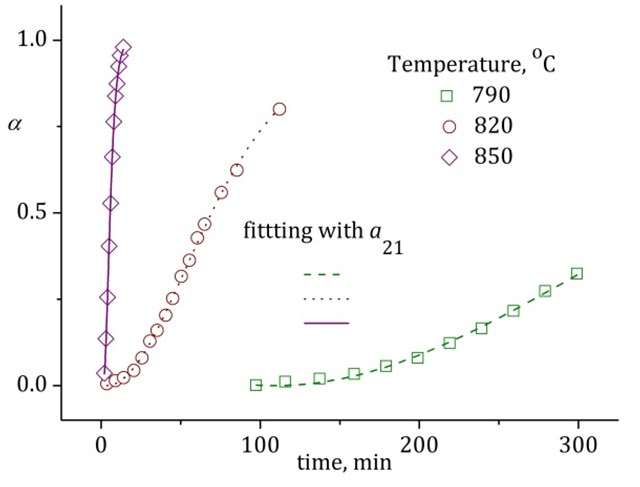
\includegraphics[width=0.83\textwidth]{min_3_curves.jpg}
    \caption{Данните от фиг. 7 на \cite{Min2005} и съответните криви с $\alpha_{21}$, с коефициент на корелация $R^2 = 0.996, 0.999, 0.999$ съответно.}
    \label{fig:a21_min}
\end{figure}

В процеса на параметрична идентификация за \autoref{fig:a21_min} получаваме скала за данните за всяка температура. Тези скали можем да използваме да преоразмерим времената от оригиналните данни. Така очакваме да получим единствена крива (т.нар. ,,master curve``) с безразмерни времена. Това ще потвърди разбирането, че режимът на растеж е един и същ и в трите случая, като данните се различават само по характеристичните времена на процеса (температурна зависимост).
\begin{figure}[hbpt]
    \centering
    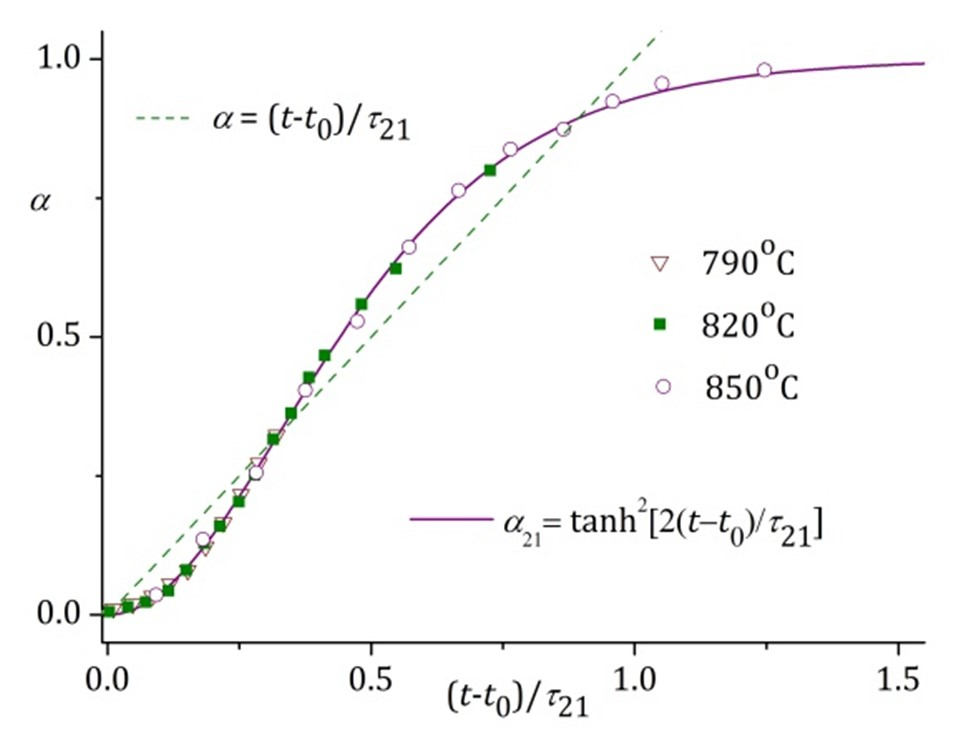
\includegraphics[width=0.65\textwidth]{min_a21_master_curve.jpg}
    \caption{Крива с рескалираните данни. Вижда се ясно как всички данни ,,лягат`` добре на една и съща крива, въпреки значително различни характеристични времена на процесите.} 
    \label{fig:a21_min_master_curve}
\end{figure}
\begin{figure}[hbpt]
    \centering
    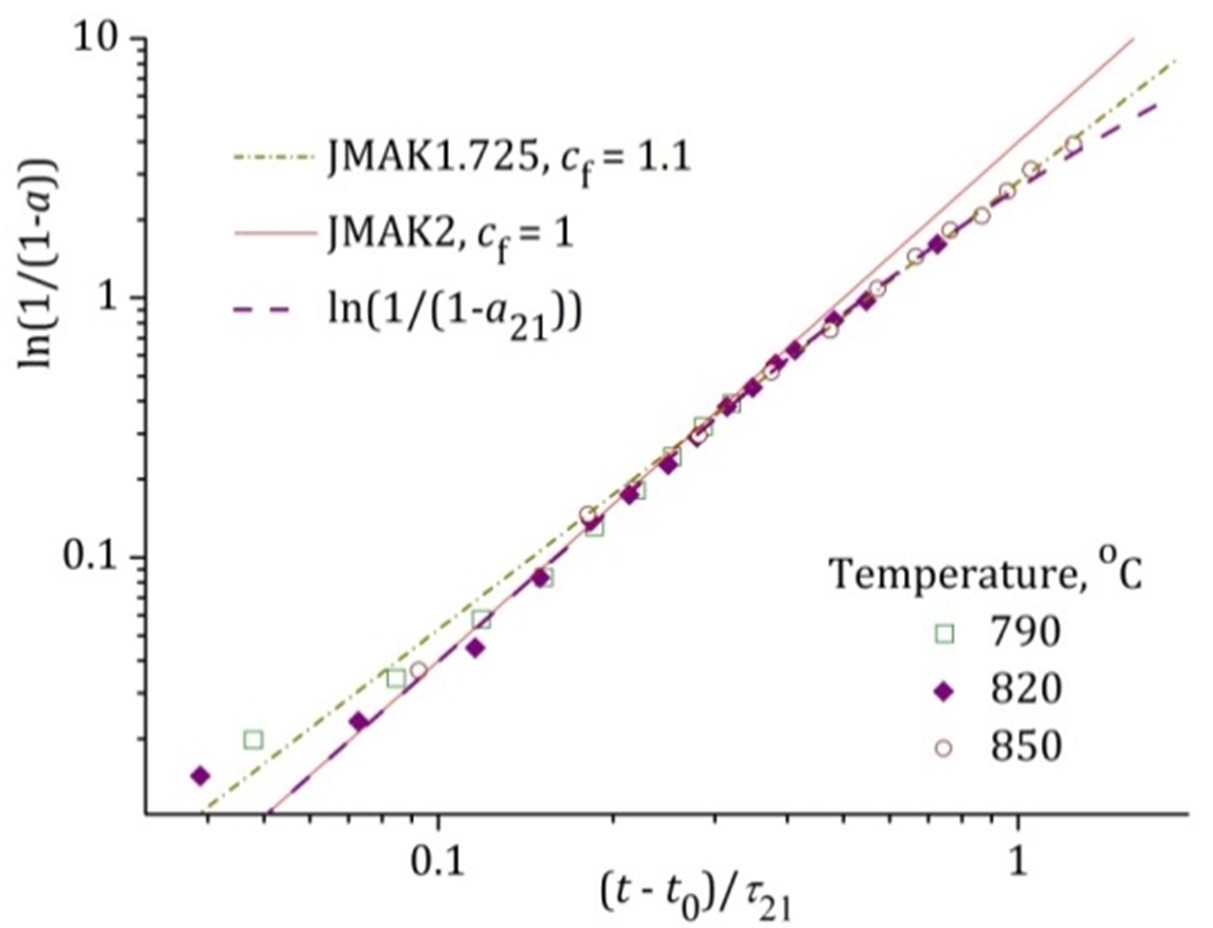
\includegraphics[width=0.65\textwidth]{min_a21_master_curve_avrami_plot.jpg}
    \caption{Крива \autoref{fig:a21_min_master_curve} представена в Аврами координати. Вижда се ясно как и при трите температури малките степени на трансформация не се описват добре от модела, но при големи $\alpha$ данните завиват надясно от JMAKn, което пък се описва добре от $\alpha_{21}$.}
    \label{fig:a21_min_master_curve_avrami}
\end{figure}

\subsection{Валидиране с данни от клетъчен автомат}
В областта на кристалния растеж един от инструментите за симулиране на физичния процес кристализация са клетъчните автомати. Те позволяват иначе сложният макроскопски процес да бъде моделиран чрез простите локални правила, които го обусловят. Един от най-първите микроскопски модели на електроотлагане на метали е така наречена дифузионно-лимитирана агрегация (DLA), чиито резултантни структури са познати като DLA-клъстери. 
\begin{figure}[hbpt]
    \centering
    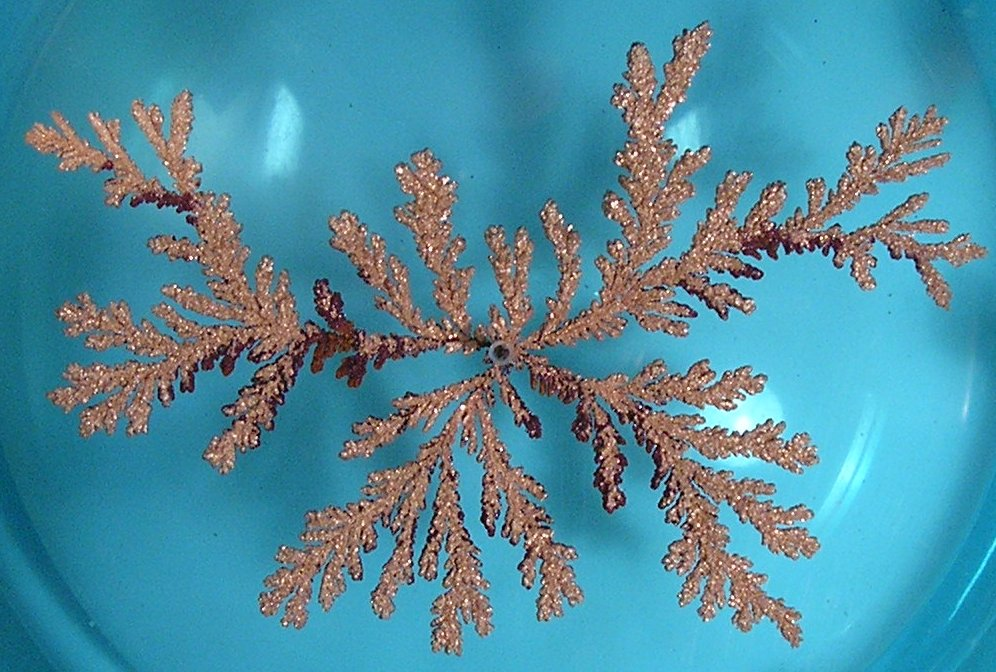
\includegraphics[width=0.65\textwidth]{dla_cluster_copper.jpg}
    \caption{DLA клъстер получен при електроотлагане на мед из разтвор на меден сулфат \cite{dla_copper}.}
    \label{fig:dla_cluster_wikimedia}
\end{figure}

Първият стохастичен (тип случайна разходка) модел на DLA е даден от \textit{Witten \& Sander} \cite{DLA_Witten}. В него започваме с агрегат от една частица (зародиша), спрямо която от ,,безкрайност`` дифундират останалите частици.
Когато една дифундираща частица пристигне при агрегата, тя се свързва необратимо като става част от него. Числената реализация на този модел има своите особености, тъй като условието за старт безкрайно далеч от агрегата е практически неизпълнимо. От друга страна, ако дифундиращите частици стартират твърде далеч от зародиша, симулациите са бавни, ако са твърде близо - предпоставки на модела се нарушават. В литературата са намерени практически решения на тези проблеми, като при симулация върху достатъчно голяма квадратна решетка се получават именно структури от вида на \autoref{fig:brownian_tree} - т.нар. браунови дървета.
\begin{figure}[hbpt]
    \centering
    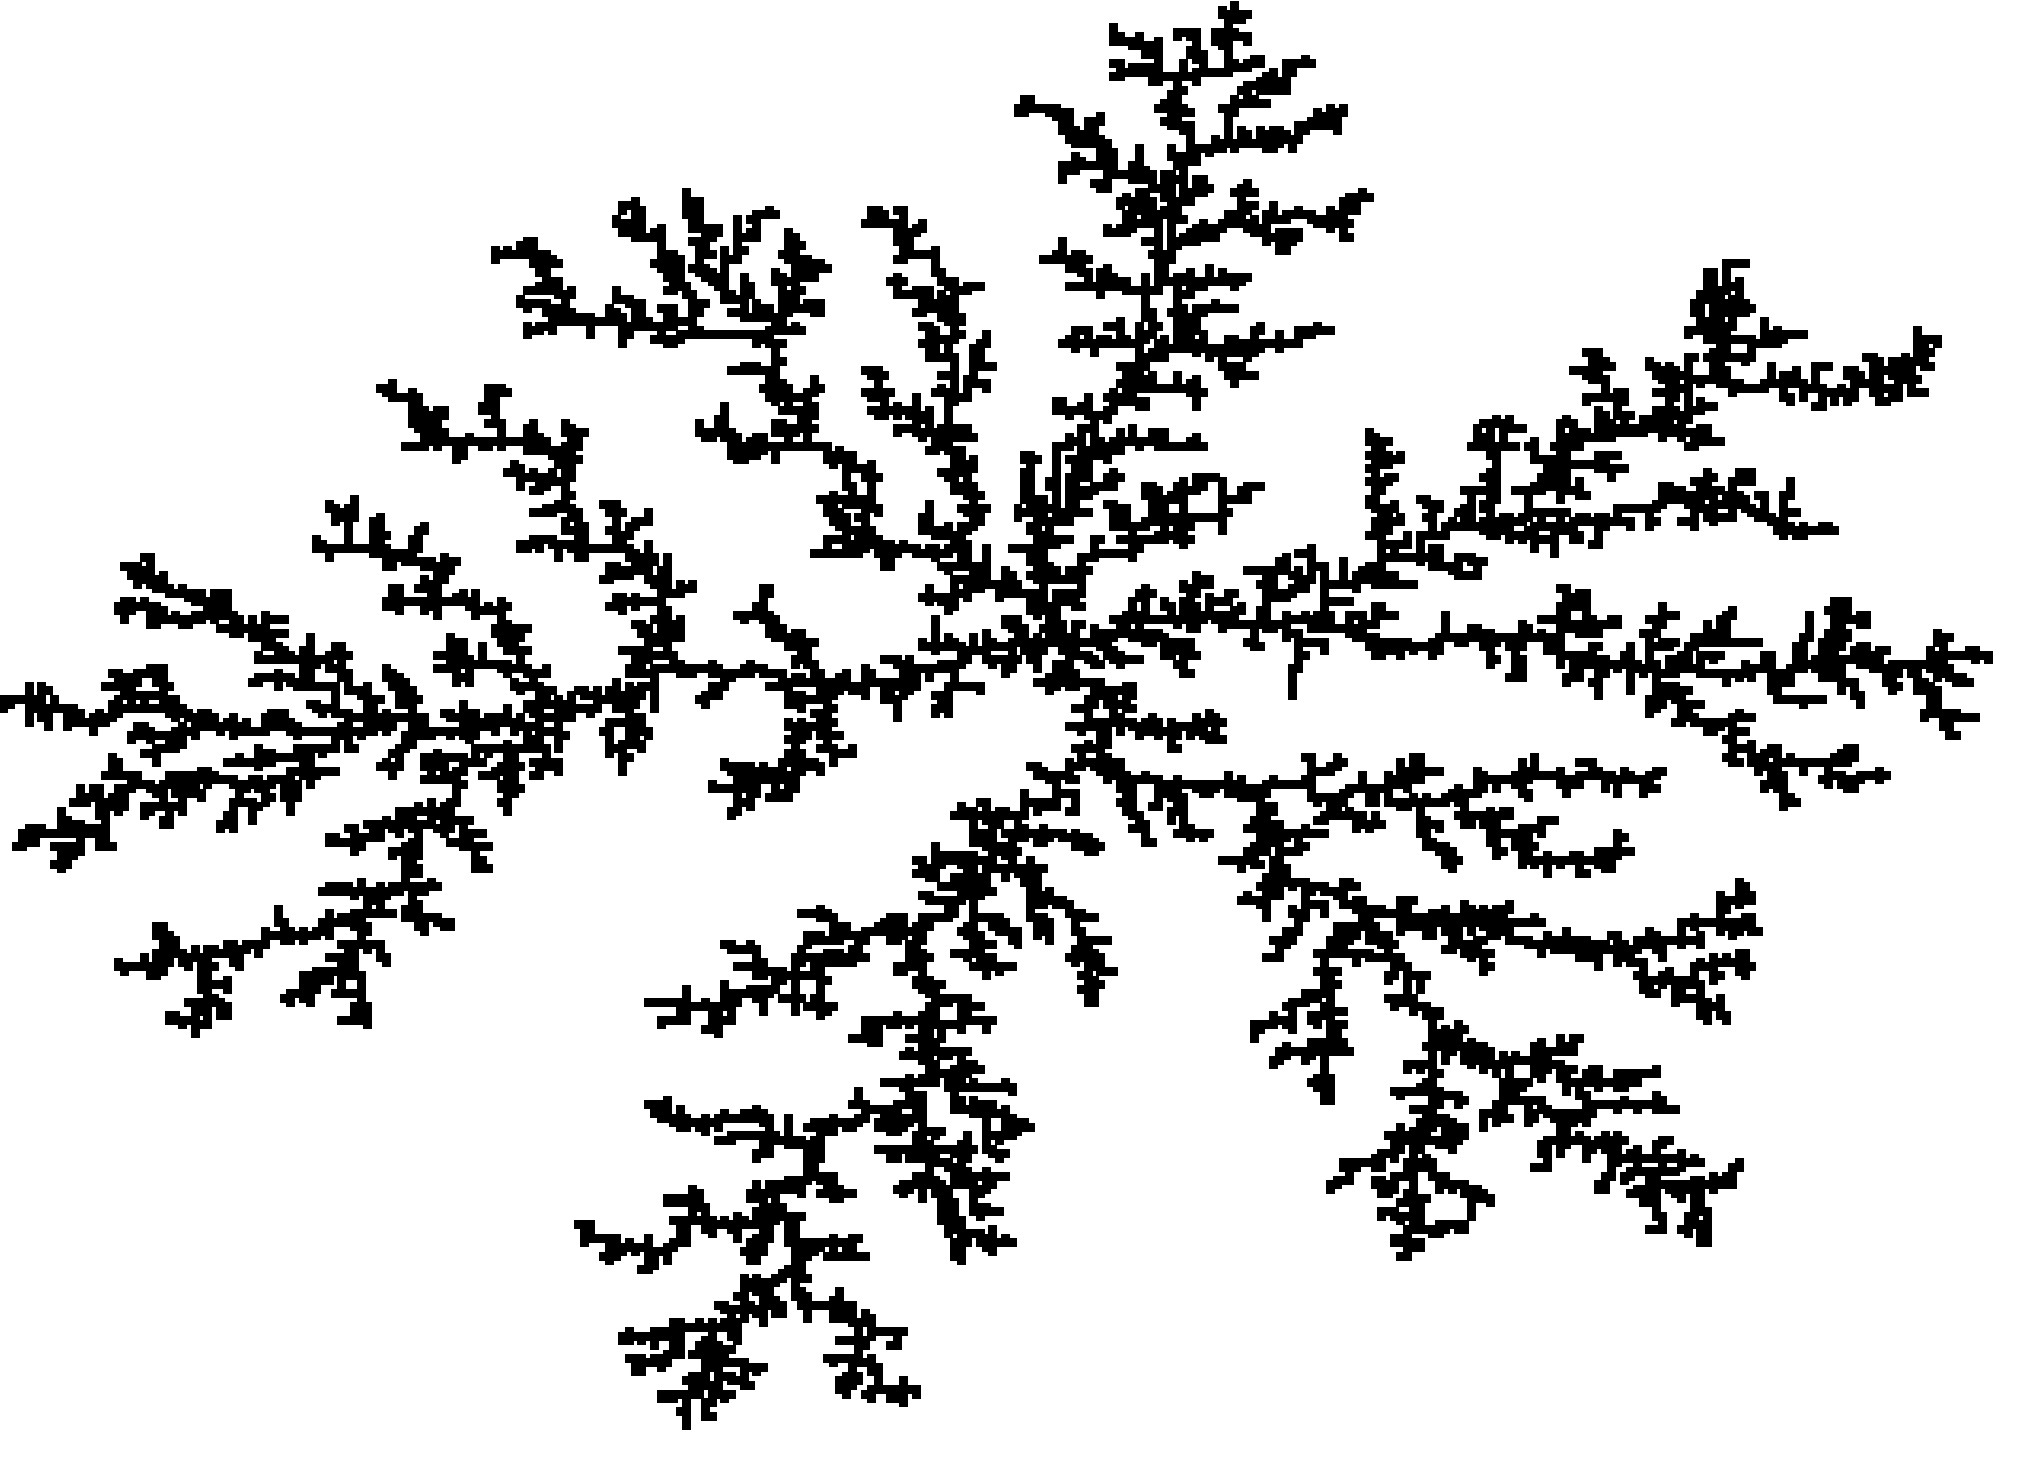
\includegraphics[width=0.65\textwidth]{brownian_tree.jpg}
    \caption{Брауново дърво получено от DLA.}
    \label{fig:brownian_tree}
\end{figure}
Допълнително от симулациите и от структурата на реалните DLA агрегати се вижда, че те имат дендритна (фрактална) структура. \textit{Menshutin} показва, че фракталната размерност на агрегата при 2D DLA е $\approx 1.7$ \cite{DLA_Menshutin}. 

DLA е добър примитивен модел, но резултатите от изследването на този модел обикновено водят до еднакво ,,рехави`` (с еднаква фрактална размерност) браунови дървета. Основните недостатъци в предпоставките му са необратимото свързване на дифундиращите частици, фиксираният им ,,дифузионен коефициент`` (винаги е 1) и малката вероятност частиците да навлязат във вътрешността на агрегата преди да се свържат. 

За целта ще построим модел на клетъчен автомат, базиран на DLA (всички позиции на свързване са еднакво енергитично изгодни - няма кинкове), който ще наречем \textit{Attachment-to-Any Cellular Automata} (A2A CA). Неговите предпоставки са следните:
\begin{enumerate}
    \item Клетките са разположени върху двумерна квадратна решетка.
    \item Всяка от тях има 3 състояния - 0 - празна, 1 - свободна (дифундираща) частица, 2 - неподвижна (в агрегата).
    \item Състоянието на една клетка се определя от \textit{четирите} ѝ най-близки съседи (околност на фон Нойман).
    \item Клетъчната колония се обновява паралелно за всички клетки по \textbf{физически съобразни правила}.
\end{enumerate}
Правилата за обновяване на колонията са следните:
\begin{itemize}
    \item Състояния 0 (празна) и 2 (агрегат) не се променят.
    \item 1 $\rightarrow$ 2 - при наличие на поне един съсед в състояние 2 (DLA правило).
\end{itemize}
Основното \textit{разширение} спрямо класическия DLA модел е, че между всеки две състояния на автомата (приложения на агрегационното правилото), обновяваме дифузионното поле серийно чрез $nds$ на брой дифузионни стъпки - частиците извършват брауново движение без да се свързват към агрегата, ако има такъв в тяхната околност. 
Ефектът от това допълнителното обновяване на дифузионното поле е, че така $nds \propto D$, където $D$-дифузионен коефициент на частиците. Допълнително от уравнението на Стокс-Айнщайн:
\begin{equation*}
    D = \frac{k_{B} T}{6 \pi \eta r} \propto T
\end{equation*}
Или $nds \propto T$, т.е. броят дифузионни стъпки моделира ефективно температурата $T$ на системата. Тази моделна система ни позволява лесно да проследим пресищането (и съответно степента на превръщане) на всяка стъпка по времето, за различни начални концентрации на дифундиращи частици, размери на решетката, $nds$ и т.н.
\begin{figure}[hbpt]
    \centering
        \subfloat[$nds = 1$]{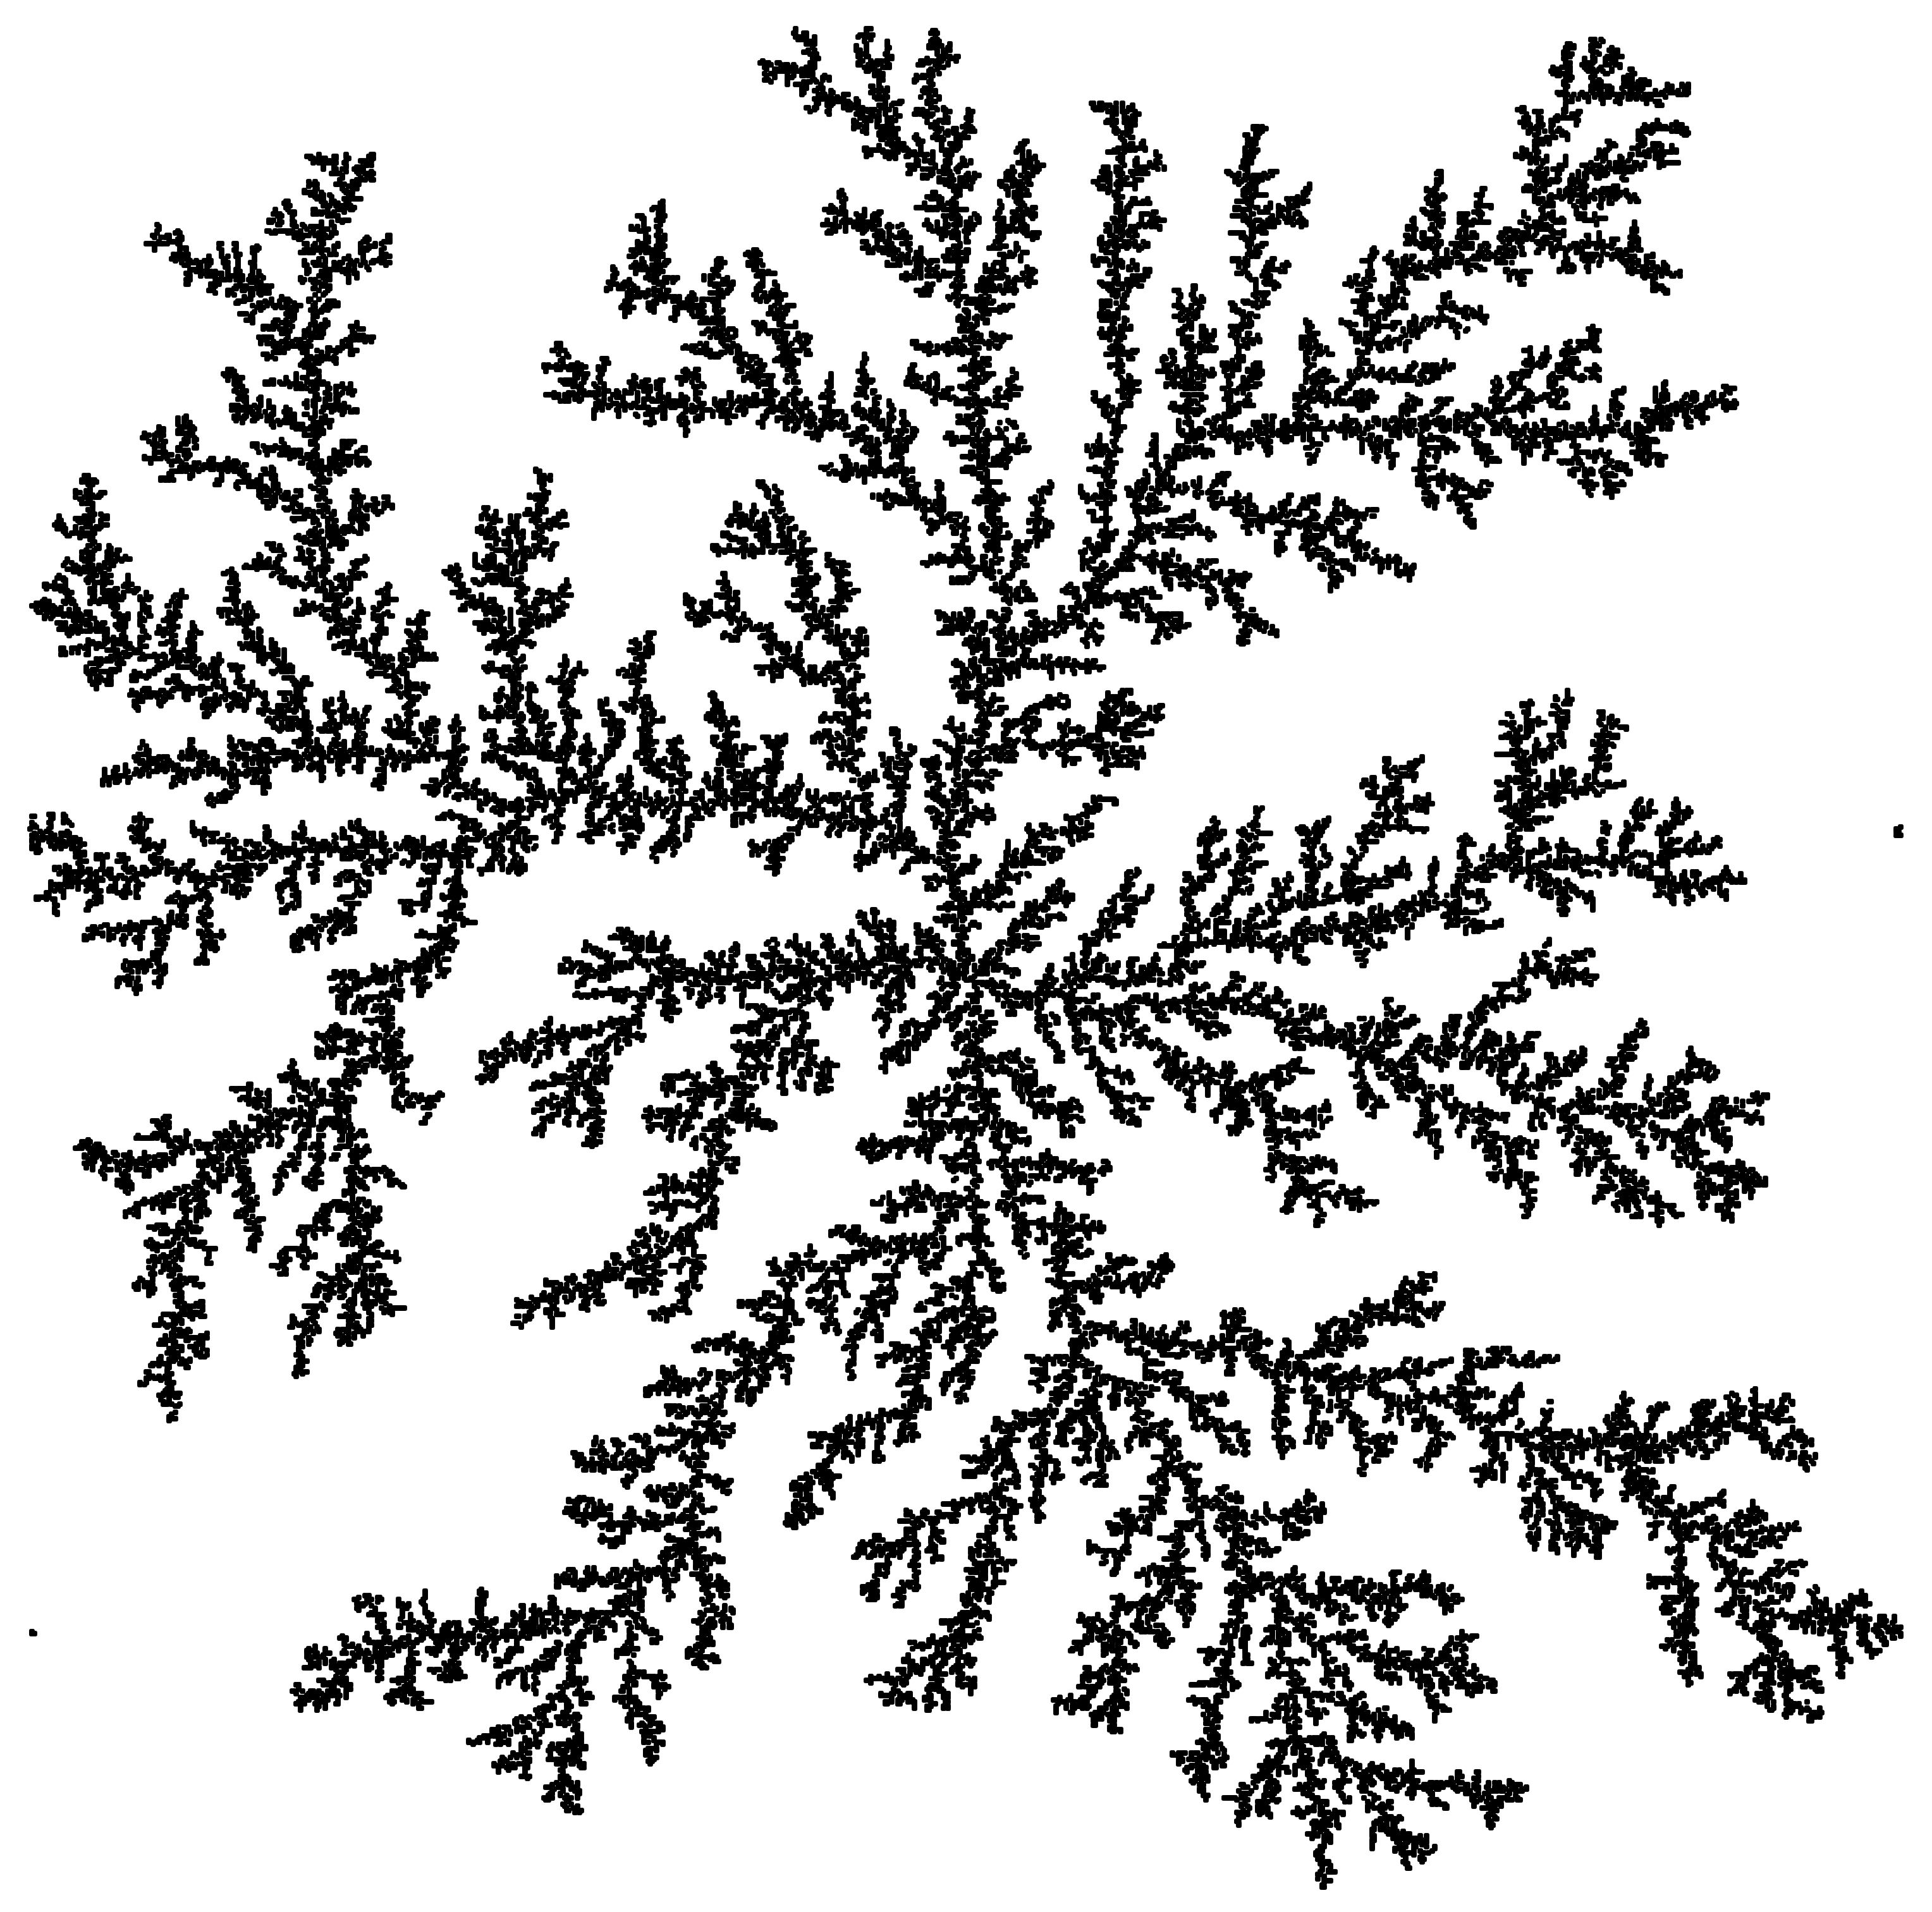
\includegraphics[width=0.43\textwidth]{nds_1_resized.png}}
        \subfloat[$nds = 200$]{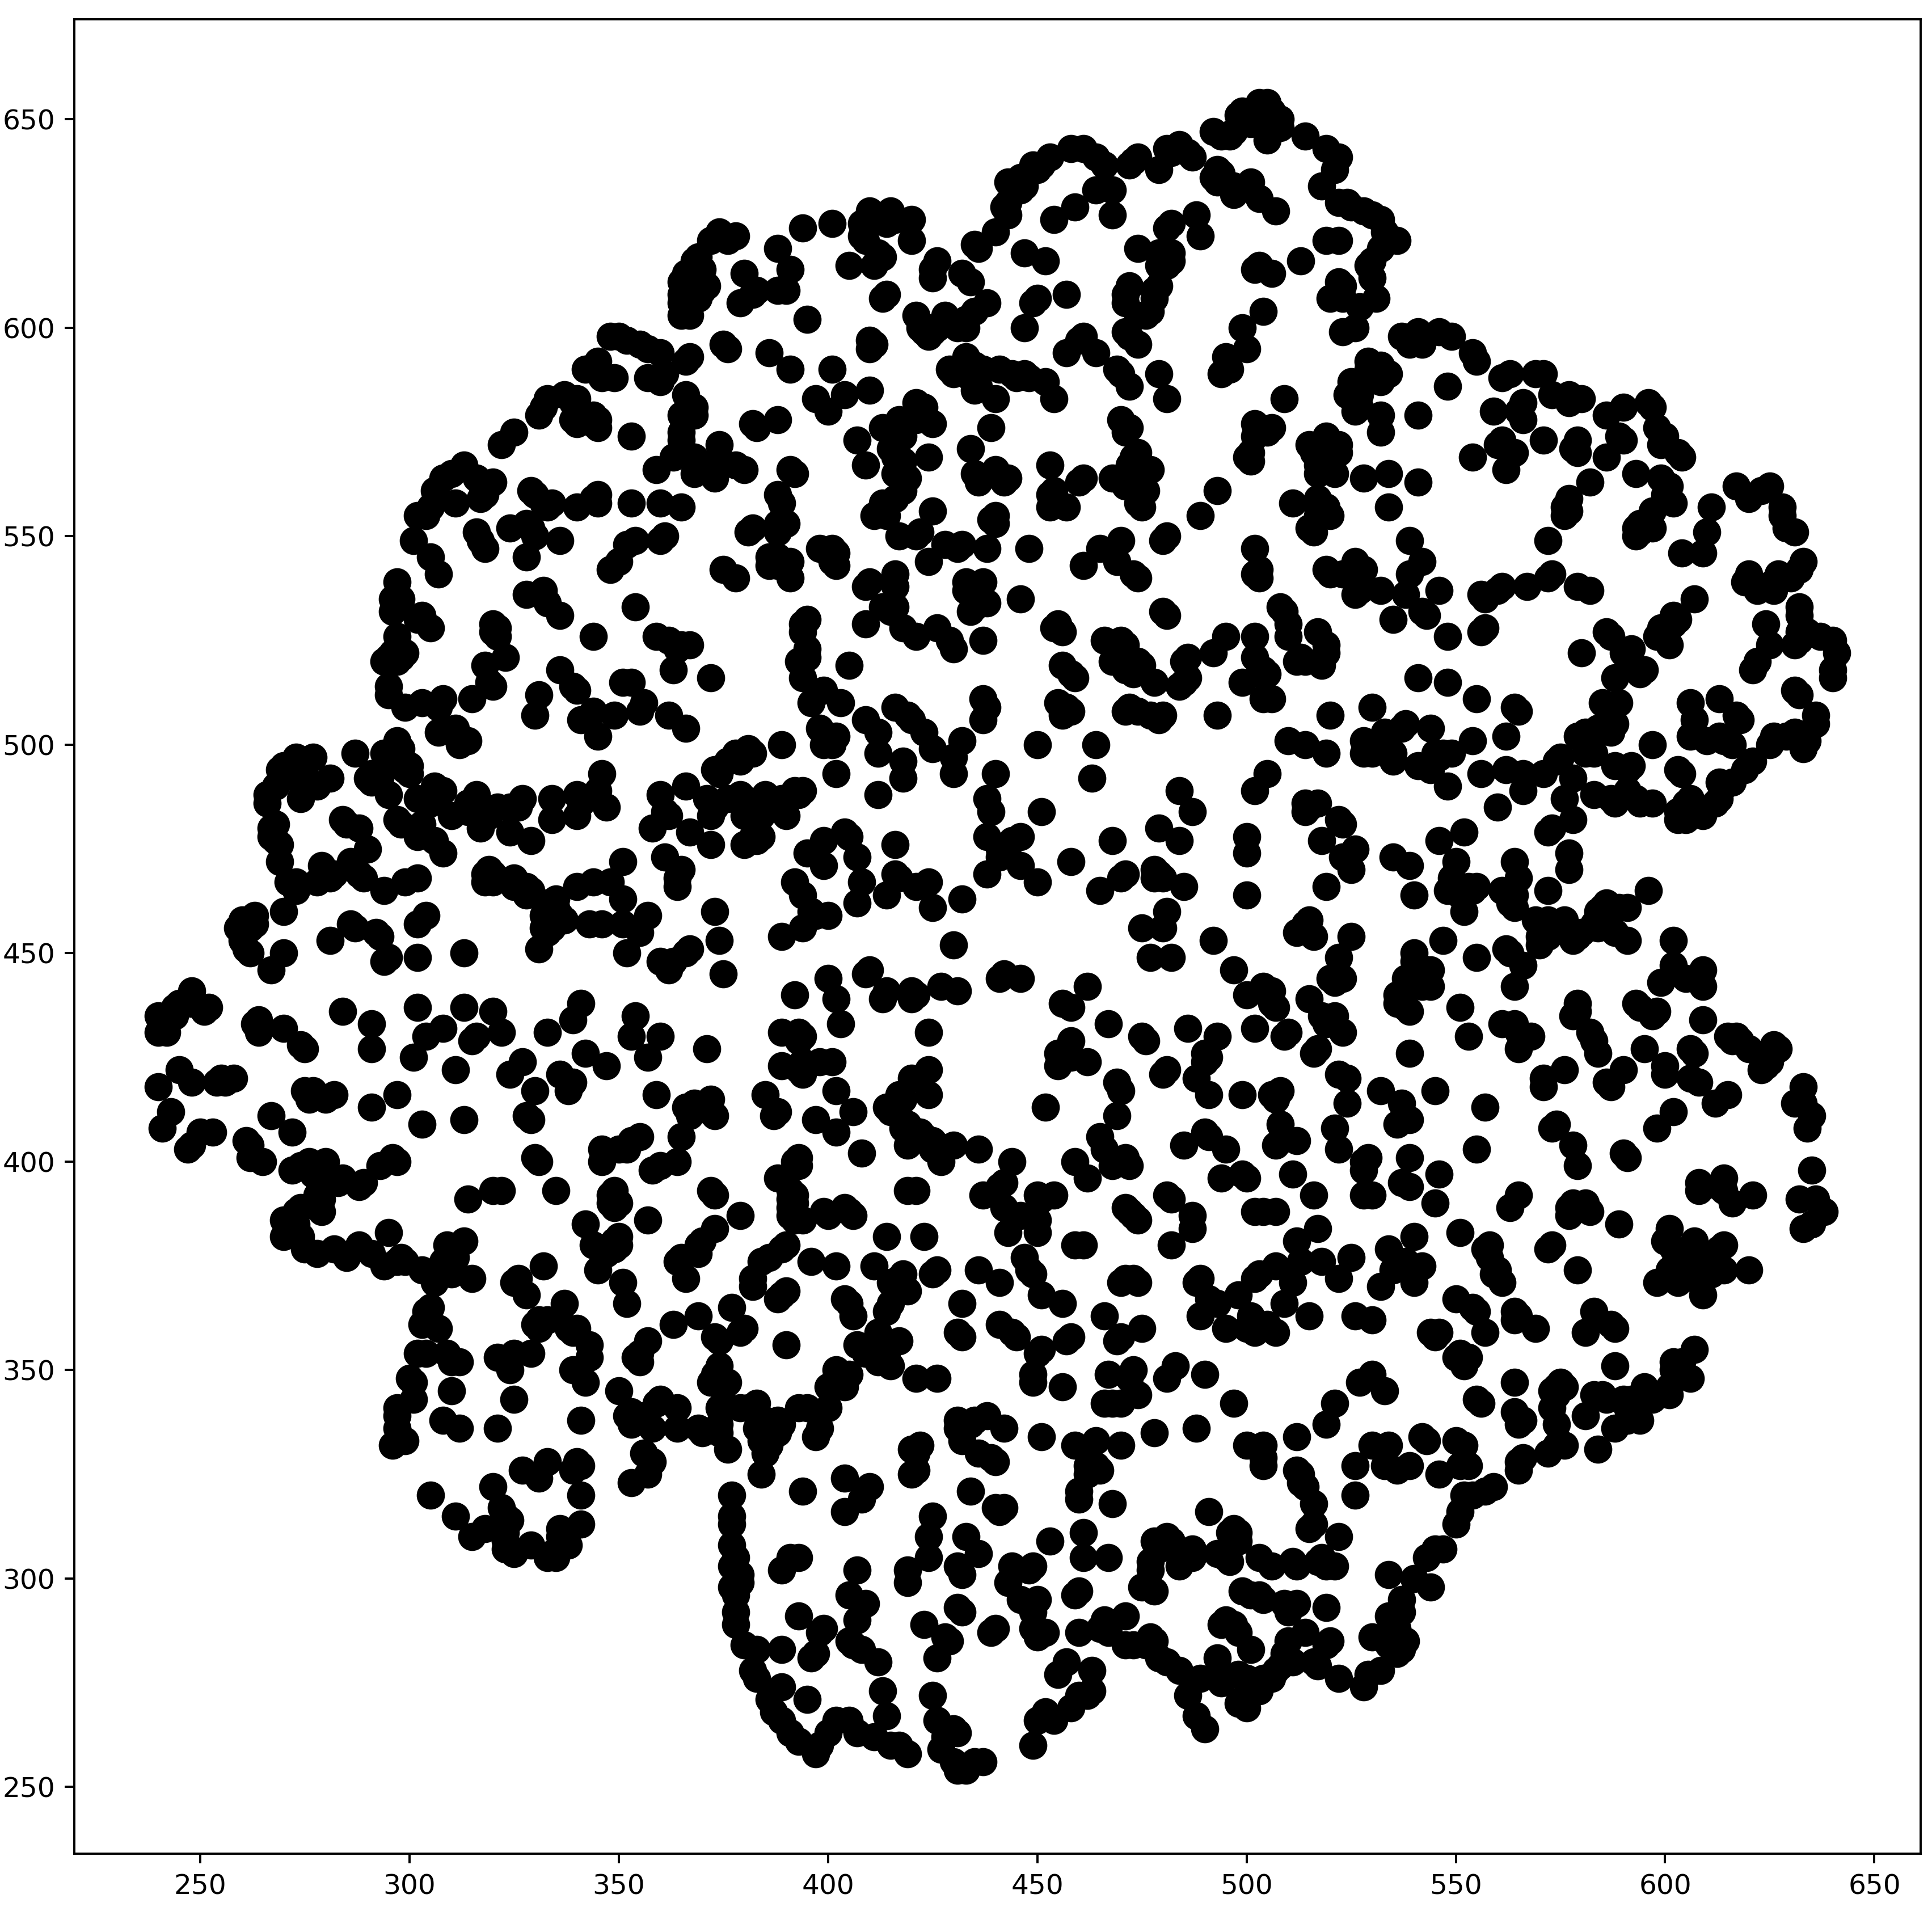
\includegraphics[width=0.43\textwidth]{nds_200_resized.png}}
    \caption{Форма на агрегата за 900x900 A2A CA при начална концентрация на дифундиращи частици c = 10\%.}
    \label{fig:nds_effect}
\end{figure}

\autoref{fig:nds_effect} демонстрира директно влиянието на различния брой стъпки на обновяване на дифузионното поле - при малки стойности на $nds$ имаме познатия от DLA агрегат, подобен на \autoref{fig:brownian_tree}, а при големи - получаваме значително по-компактна структура, с граница много по-близо до кръг. Допълнително, и за двата агрегата от крайната им структура не можем да разпознаем симетрията на решетката върху която са раснали (квадратна), т.е. в една по-разширена версия на такъв клетъчен автомат, в която са моделирани и кинк позициите бихме искали да получим и този ефект на възпроизвеждане на пространствената симетрия на система в крайната структура. За настоящата цел на валидиране на $\aDg$, А2А CA все пак е достатъчно подробен модел.

Протоколът на числения експеримент ще бъде следния: Фиксираме размера на решетката на 900x900 и изследваме \textit{c = 0.025, 0.040, 0.055, 0.070, 0.085, 0.100, 0.115, 0.130} и \textit{nds = 1, 2, 4, 6, 8, 10, 25, 50, 100, 150, 200}. За всяка комбинация $(c, nds)$ правим по 4 старта (4 различни агрегата) на A2A CA. Общо, това са $8 \times 11 \times 4  = 352$ набора данни за степента на трансформация $(t^i, \alpha^i)$. За да намалим количеството данни, които трябва да обработваме, за дадена комбинация $(c, nds)$ ще усредим $\alpha - t$ кривите по агрегатите.

Тъй като тук предпоставката е за дифузионен контрол, фиксираме $g = 1$. При изследване на $D$, което получаваме от оптимизационната процедура резултатите са $D \in [1.67, 2.2]$. По тази причина отново ще фиксираме $D = 2, g = 1$, за да работим директно с $\alpha_{21}$. Ще изследваме подробно как скалата $\tau_{21}$ зависи от $nds$ и още повече - как скейлинговата експонента $\kappa$ от $\tau_{21} \propto nds^\kappa$ зависи от концентрацията $c$.

За да можем да получим експонентата $\kappa$ ще разгледаме в $\log-\log$ зависимостта на $\tau_{21}$ от $nds$.
\begin{figure}[hbpt]
    \centering
    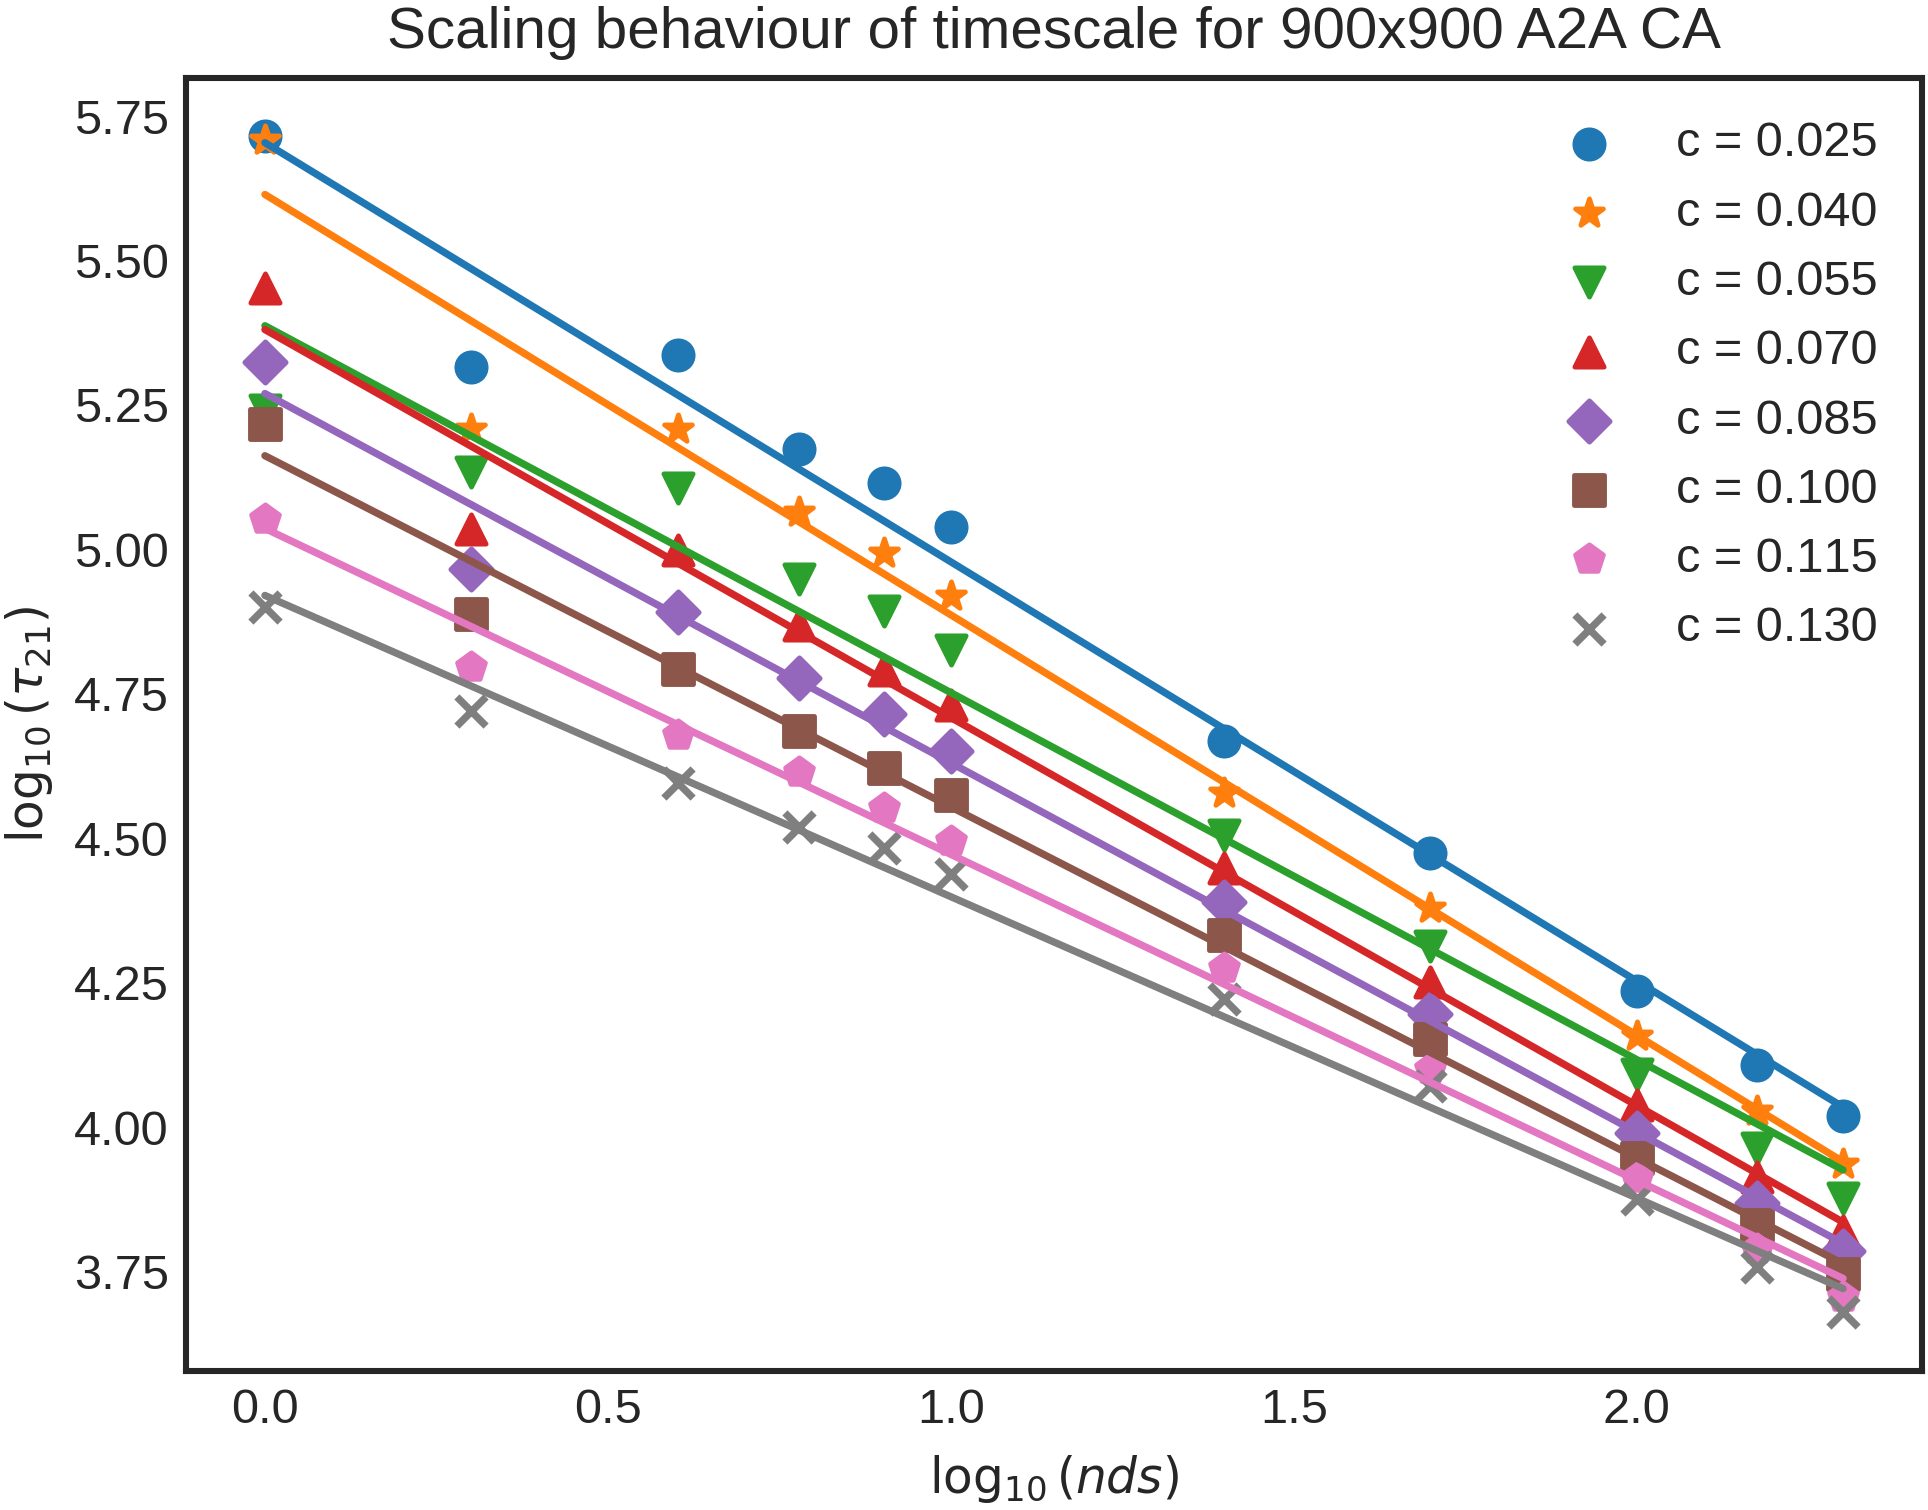
\includegraphics[width=0.85\textwidth]{scaling_plot_all_a2a_ca.png}
    \caption{Скейлинг на $\tau_{21}$ с $nds$}
    \label{fig:scaling_tau21_nds}
\end{figure}
\begin{table}[hbpt]
\centering
\caption{Резултати от линейната регресия за всяка от концентрациите на автомата.}
\label{tabl:scaling_tau21_nds}
\resizebox{0.65\textwidth}{!}{%
\begin{tabular}{@{}cccc@{}}
\toprule
Концентрация ($c$) & Наклон $(\kappa)$    & Отрез    & $R^2$    \\ \midrule
0.025        & -0.725204 & 5.703861 & 0.986310 \\
0.040        & -0.727381 & 5.614268 & 0.985010 \\
0.055        & -0.634860 & 5.387181 & 0.977654 \\
0.070        & -0.671192 & 5.380443 & 0.989942 \\
0.085        & -0.639080 & 5.269890 & 0.993133 \\
0.100        & -0.607593 & 5.162227 & 0.994085 \\
0.115        & -0.563946 & 5.036357 & 0.994955 \\
0.130        & -0.521279 & 4.920473 & 0.993984 \\ \bottomrule
\end{tabular}%
}
\end{table}

\autoref{fig:scaling_tau21_nds} и \autoref{tabl:scaling_tau21_nds} потвърждават очакванията за температурната зависимост на $\tau_{21}$ - с увеличаване на температурата процесът на агрегация (кристализация) се ускорява и съответно характеристичното му време намалява.

Наклонът на регресионните прави от \autoref{tabl:scaling_tau21_nds} е експонентата $\kappa$, докато отрезът е характеристичното време при $nds = 1$. Намаляването на $\tau$ с $nds$ е относително ,,бавно`` - два порядъка промяна по $nds$ водят до по-малко от два порядъка намаляване на характеристично време за всяка от концентрациите.

\begin{figure}[H]
    \centering
    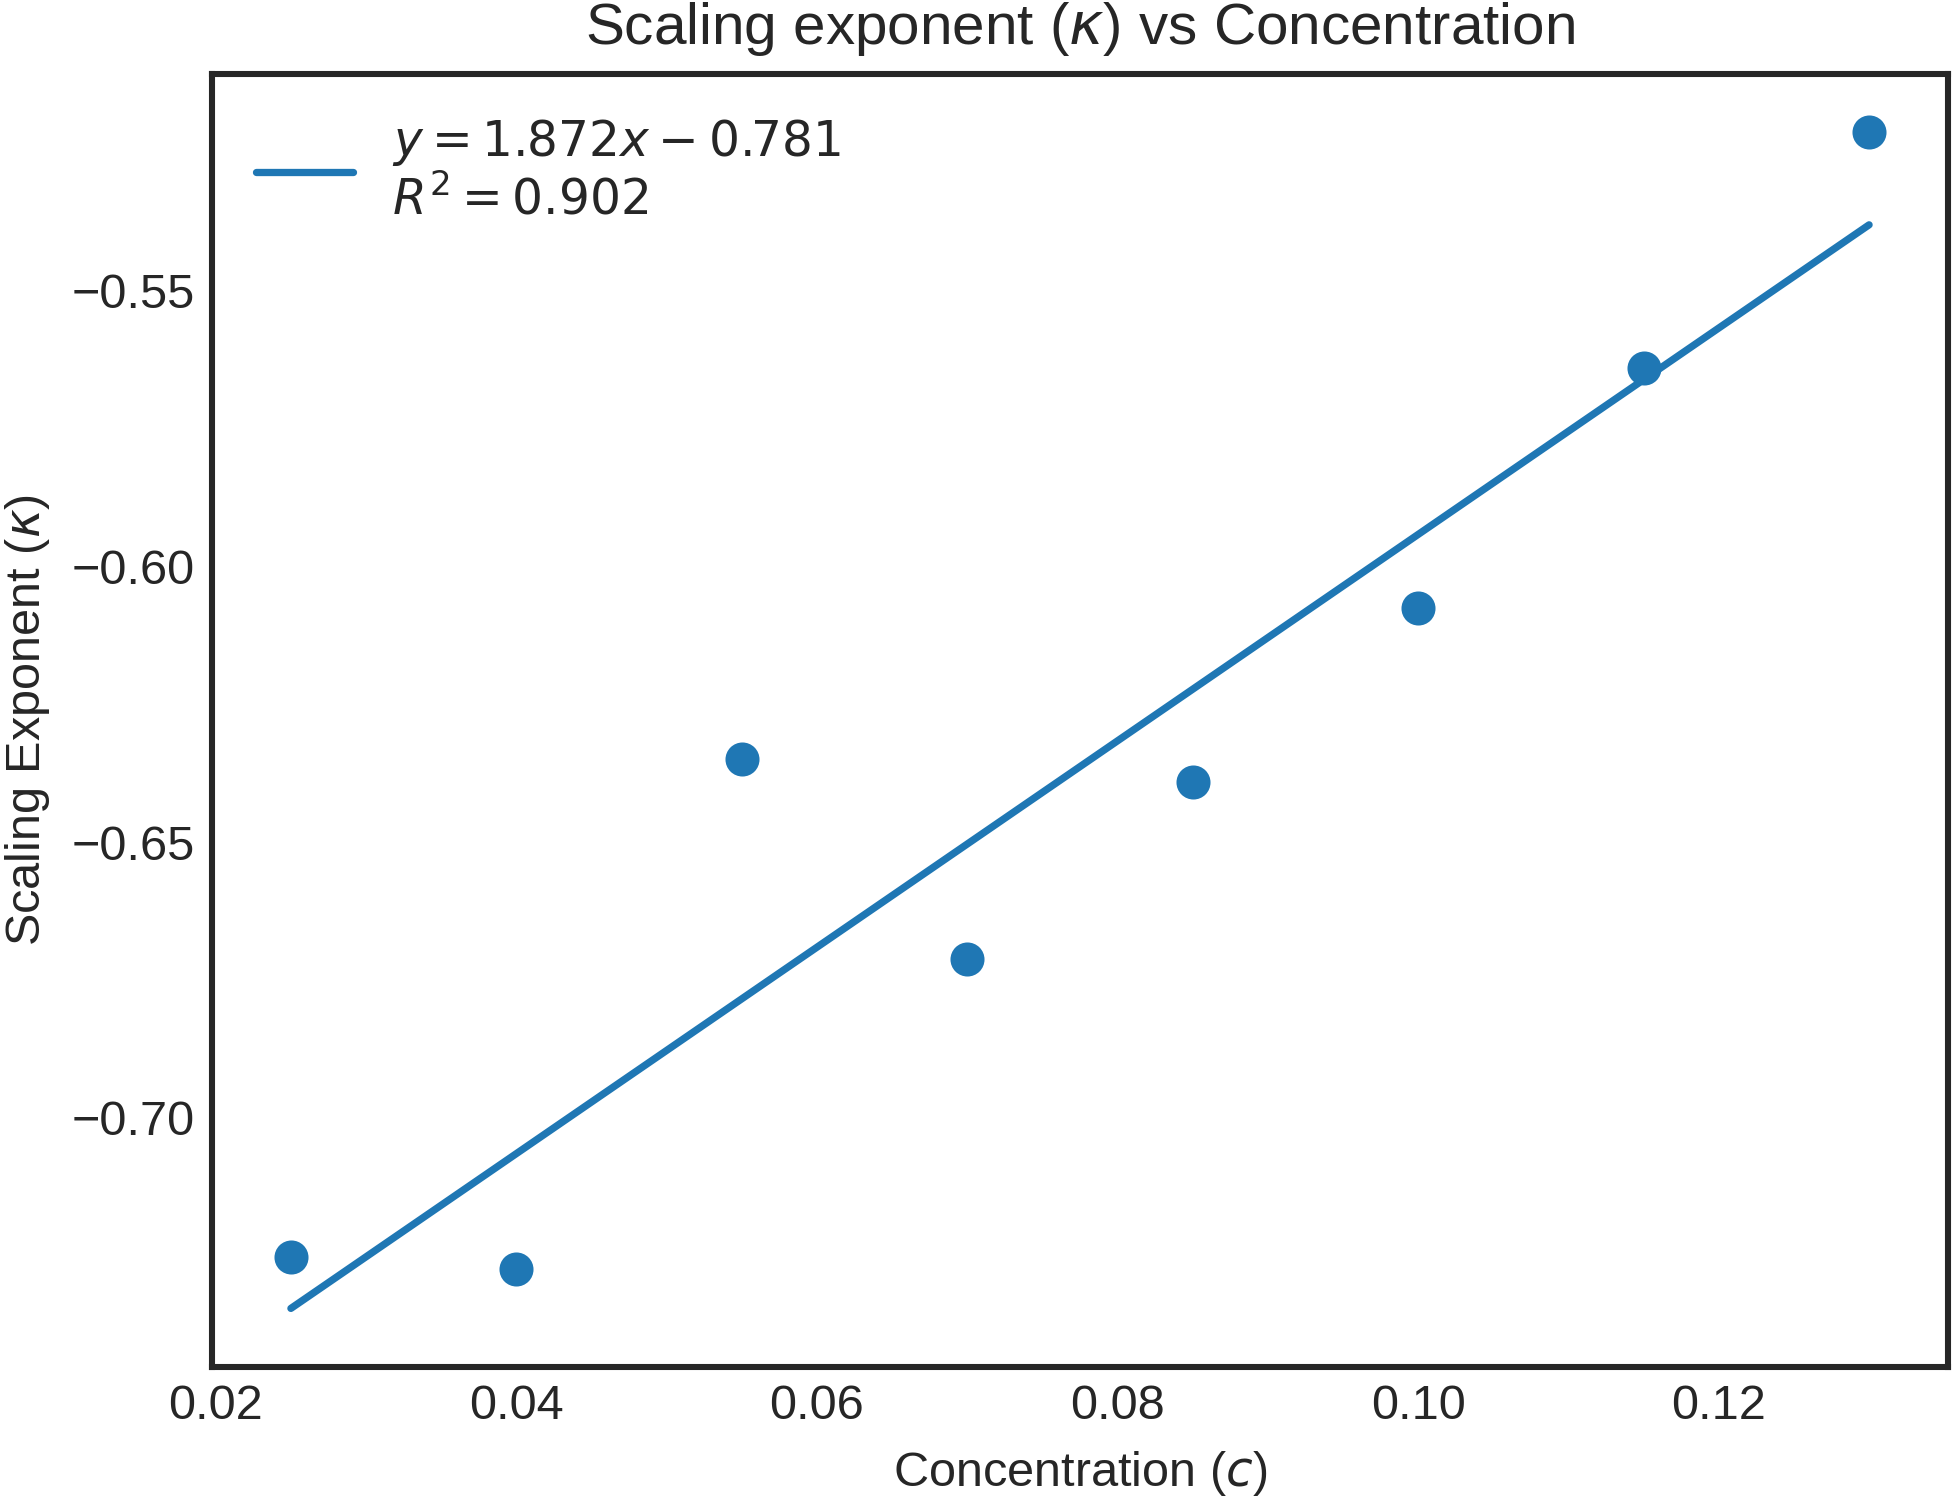
\includegraphics[width=0.7\textwidth]{slope_vs_conc.png}
    \caption{Зависимост на експонентата $\kappa$ от концентрацията $c$}
    \label{fig:scaling_kappa_vs_conc_ca}
\end{figure}

В \autoref{tabl:scaling_tau21_nds} има генерална тенденция $\kappa$ да нараства с концентрацията. За целта на \autoref{fig:scaling_kappa_vs_conc_ca} е изследвана именно тази зависимост. Тук линейната зависимост не е толкова недвусмислена, както при \autoref{fig:scaling_tau21_nds},но въпреки това очертава общата тенденция на нарастване на $\kappa$ в този интервал от концентрации, както и поставя въпроса (при екстраполация) как би изглеждала граничната стойност на $\kappa^0 = \kappa (c \rightarrow 0)$. Тъй като $\kappa ^ 0$ би било трудно да се оправдае физически (при липса на частици - не се образува агрегат), би следвало преди да си позволим такива разсъждения да изследваме поведението на все ,,по-разреден`` A2A CA.

\subsection{Обобщение на резултатите за модела} 
От валидиране с данните на \textit{Min, Sinclair, et. al.} \cite{Min2005} беше показана силата на $\aDg$ модела да описва експерименти, които JMAKn не може да обясни. Показано беше, че точките с най-голяма дискриминативна сила за двата модела са тези при големи степени на превръщане ($\alpha \rightarrow 1$), близки до равновесието. Това противоречи на пряката интуиция, защото бихме очаквали близо до равновесието всички разлики в режима на растеж да са ,,изгладени`` и детайлите на механизма да са ,,загубени``, а точно тези части на процеса се оказват най-характеристични. От експерименталните данни в предния параграф видяхме, че завиването надясно в Аврами координати е физически важно.

Валидирането с данните от симулация на A2A CA поставят $\aDg$ модела като добър инструмент за изследване на температурната зависимост на различни системи на агрегация и кристализация. A2A CA ни позволяват да генерираме много повече данни, с които да изследваме поведението на модела и моделните системи, отколкото би било практически постижимо при изследване на такива реални системи.

Можем да дадем следната ,,рецепта``, която да се прилага за $\aDg$:
Единият подход е да използваме директно числените процедури от \autoref{subsub:parametric_identification} и ако получените параметри са близки до цели числа, ги закръгляваме до съответното най-близко цяло, избираме съответната аналитична крива и правим параметрична идентификация за времевата скала. Ако получените параметри са извън $ 0.5 \le D \le 3.5$ и $0.5 \le g \le 2.5$ считаме, че данните не могат да бъдат обяснени с модела. 

Аналогично, когато сме сигурни, че имаме режим на дифузионен контрол, т.е. $g = 1$, можем да направим параметрична идентификация за $n$, $\tau$ от JMAKn, тъй като там имаме общ аналитичен израз. От уравнението на \autoref{fig:nvsd_graph} за полученото $n$ избираме $D$ и го закръгляваме. Нататък повтаряме предната процедура.

Ако при всеки от двата подхода за избраната $\aDg$-крива коефициентът на Пиърсън $R^2$ е малък, също считаме че моделът не може да обясни добре наблюдавания експеримент.

Тези ограничения върху целите стойности може да изглеждат ненужни и твърде строги, особено с процедурите от \autoref{subsub:parametric_identification}. Ние обаче ги налагаме така щото да държим сметка за началните предположения, при които е изведен модела, за да може те да имат ясен физичен смисъл. 
С използването на модела и задълбочаването на познаването му в контекста на различни експериментални данни, можем да си позволим да освободим размерността да бъде реално число, т.е. да твърдим че $D$ e фракталната размерност на растящия кристал. Такава ретроактивна промяна на смисъла на един параметър трябва да бъде направена внимателно, само когато са на лице подходящи експерименти, с които тази хипотеза да бъде изследвана. Такъв числен експеримент би бил например клетъчен автомат, растящ послойно от 2D към 3D. Ако получаващите се стойности от \textit{NLSQ/Uniform} корелират с фракталната размерност на автомата, то бихме могли да направим такава рационализация за $D$.